\documentclass[11pt,a4paper]{report}

% Aberstwyth dissertation LaTeX Template
% Authors: Dr. Hannah Dee (hmd1@aber.ac.uk), Neil Taylor (nst@aber.ac.uk)
% This has been adapted from the Leeds Thesis template and the 
% Group Project template for Computer Science in Aberystywth University.
% 
% All comments and suggestions welcome.
%
% Template designed to be used with pdflatex: it may need alteration to
% run with a different LaTeX engine

% To build document on the unix command line, run four commands:
 
% pdflatex dissertation
% bibtex dissertation
% pdflatex dissertation
% pdflatex dissertation

% you will end up with dissertation.pdf 
\usepackage{mmp}

% the following packages are used for citations - You only need to include one. 
%
% Use the cite package if you are using the numeric style (e.g. IEEEannot). 
% Use the natbib package if you are using the author-date style (e.g. authordate2annot). 
% Only use one of these and comment out the other one. 
\usepackage{cite}
%\usepackage{natbib}

\usepackage{titlesec}

% Use the following to selectively exclude chapters
%\includeonly{cover,abstract,acknowledge,declare,chapter1,chapter2}

\begin{document}

% all of the include directives below refer to tex files
% so 
\title{Location Sensitive Social Notifier}

% Your name
\author{Thomas Mark Rosier}

% Your email 
\authoremail{thr2@aber.ac.uk}

\degreeschemecode{G600} %e.g. G400 
\degreeschemetitle{Software Engineering} % e.g. Computer Science
\degreetype{BEng}

\modulecode{CS39440} % i.e. CS39440, CC39440, CS39620
\moduletitle{Major Project} % i.e. Major Project or Minor Project

\date{\today} % i.e. the date of this version of the report

\status{Release} % Use draft until you create the release version. Then, change this to Release.
\version{1.0}

%The title and name of your supervisor.
\supervisor{David Ernest Price} 

%The email for your supervisor. 
\supervisoremail{dap@aber.ac.uk}

\maketitle



 includes cover.tex - to change the content,
% edit the tex file

\pagenumbering{roman}

% This is the front page

\title{Location Sensitive Social Notifier}

% Your name
\author{Thomas Mark Rosier}

% Your email 
\authoremail{thr2@aber.ac.uk}

\degreeschemecode{G600} %e.g. G400 
\degreeschemetitle{Software Engineering} % e.g. Computer Science
\degreetype{BEng}

\modulecode{CS39440} % i.e. CS39440, CC39440, CS39620
\moduletitle{Major Project} % i.e. Major Project or Minor Project

\date{\today} % i.e. the date of this version of the report

\status{Release} % Use draft until you create the release version. Then, change this to Release.
\version{1.0}

%The title and name of your supervisor.
\supervisor{David Ernest Price} 

%The email for your supervisor. 
\supervisoremail{dap@aber.ac.uk}

\maketitle



                        

% Set up page numbering
\pagestyle{empty}

% declarations of originality 
\thispagestyle{empty}

%%%
%%% You must sign the declaration of originality. 
%%%
\begin{center}
    {\LARGE\bf Declaration of originality}
\end{center}
In signing below, I confirm that:

\begin{itemize}
\item{This submission is my own work, except where clearly
indicated.  }

\item{I understand that there are severe penalties for plagiarism 
and other unfair practice, which can lead to loss of marks
or even the withholding of a degree. }
 
\item{I have read the sections on unfair practice in the Students' 
Examinations Handbook and the relevant sections of the 
current Student Handbook of the Department of Computer 
Science.}
 
\item{I understand and agree to abide by the University's
regulations governing these issues.}
\end{itemize}

\vspace{3em}
Signature ............................................................  \\

\vspace{1em}
Date ............................................................ \\

%%% 
%%% We would like to make a selection of final reports available to students that take 
%%% this module in future years. To enable us to do this, we require your consent. You 
%%% are not required that you do this, but if you do give your consent, then we will have 
%%% the option to select yours as one of a number of reports as examples for other 
%%% students. If you would like to give your consent, then please include the following 
%%% text and sign below. If you do not wish to give your consent, please remove this 
%%% from your report. 
%%%
\vspace{5em}
\begin{center}
    {\LARGE\bf Consent to share this work}
\end{center}
In signing below, I hereby agree to this dissertation being made available to other
students and academic staff of the Aberystwyth Computer Science Department.  

\vspace{3em}
Signature ............................................................  \\

\vspace{1em}
Date ............................................................ \\

               

\thispagestyle{empty}

\begin{center}
{\LARGE\bf Acknowledgements}

I would like to dedicate my dissertation to Linda Hatfield, My great aunt who has helped with moral support and encouragement throughout my degree her kind words have kept me determined to achieve the goal of completing this degree.

% Family
Next I would like to acknowledge and my family my parents for raising me and supporting me whilst giving me the opportunity to do a degree in a subject that I am passionate.

Angela \& Mark Rosier

My brothers and there partners for being there throughout:

\begin{tabular}{ l r }
Jonathan \& Eleri Rosier & Matthew Rosier \& Stephine Fruen.\\
\end{tabular}

\begin{tabular}{ l r }
Daniel Brothers & Claire Mollart\\
\end{tabular}

% Oracle
I would like to acknowledged my former coworkers and friends from Oracle for there input and support throughout my industrial placement and the early formations of the idea for this project.

\begin{tabular}{ l c r }
Peter Woodward & James Atkinson & James Maher\\
\end{tabular}

% Old buddies
\begin{tabular}{ l r }
Karl Brown & Cian O'Shaughnessy\\
\end{tabular}

% Others Aber people
\begin{tabular}{ l c c r }
Charlotte Ford & Daniel Jones & Thomas Nicolaides & Chloe Major\\
\end{tabular}

% Staff

\begin{tabular}{ l r }
Alison Nash & Mary Glasser\\
\end{tabular}

% Main Comp Sci
I would like to thank all of my fellow Computer Science students the following are honorable mentions as they have been great friends: 

\begin{tabular}{ l c c r }
Samuel Sherar & Samuel Clements & Samuel Nicholls & Samuel Jackson \\
Alexander Stuart & Victoria Haxness & Natalia Miller & Helen Harman \\
Christopher Savill & Christopher Marriott & Roberto Fajardo & Jonathon Shire \\
Gavin Wilson & Andrew Cooper & Scott Roe & Nicholas Pattern \\ 
\end{tabular}

Last but not least I would like to thank the following teaching fellows and lecturers for there help and advice throughout this project:

\begin{tabular}{ l c c r }
Neil Taylor & David Price & Christopher Loftus & Andrew Starr\\
\end{tabular}

Thank you for the 4 best years of my life.
\end{center} % Acknowledgements
\thispagestyle{empty}

\begin{center}
    {\LARGE\bf Abstract}
\end{center}

\noindent
The aim of Location Sensitive Social Notifier is to give a platform for location based messaging, which should enable members of the public or companies to portray messages that then can be viewed when an individual is near to the message. This is a lucrative platform that could be used between friends or as a advertising platform for companies that want to sales there wears, there are many possibilities for the application many of which we do not know yet each user will find there own unique niche to fill with the application.\\
\\
The project aims to create a platform that requires no extra hardware and that can be run from a standard Google Android smart phone with just the use of GPS to determine where the device is placed. Platform wise the project uses a mixture of the stock Android SDK \cite{Google:androidAPIDocs:2015:online} for the front end application, Node.js\cite{nodeteam:node:2015:online} with the HAPI.js\cite{hapiteam:hapti:2015:online} framework for the middle tier application and a PostgreSQL\cite{Postgres:APIDocumentation:2015:online} database for the database tier of the application. With the use of advanced GPS tracking the application can detect when there is a message near by to the user and ping up a notification within the Google Android UI to notify the user of the near by message which they can then interact with by either commenting or voting on the message that been left this should engage a community atmosphere around messages.\\ 
\\
Soon Location Sensitive Social Notifier will be available on the Google Play Store and the platform will be available to millions of possible users this will hopefully be a very exciting platform that allows users to share messages and will grow into a interesting community that people want to be apart of.                 % Abstract

\setcounter{secnumdepth}{4}

\titleformat{\paragraph}
{\normalfont\normalsize\bfseries}{\theparagraph}{1em}{}
\titlespacing*{\paragraph}
{0pt}{3.25ex plus 1ex minus .2ex}{1.5ex plus .2ex}

\pagenumbering{roman}
\pagestyle{fancy}
\fancyhead{}
\fancyfoot[C]{\thepage}
\renewcommand{\headrulewidth}{0 pt}
\renewcommand{\chaptermark}[1]{\markboth{#1}{}}

\tableofcontents   
\newpage
\listoffigures
\newpage 
\listoftables
\newpage

% Set up page numbering
\pagenumbering{arabic}

\setchapterheaderfooter

% include the chapters
\chapter{Background \& Objectives}

The primary goal of this project was to create a fun and interesting manor to send messages between friends, while trying to design and implement something new and ingenuity.\\
\\
Location Sensitive Social Notifier or Lo Se Sono for short offers the opportunity to be a completely new platform to communicate messages between people and be a potential public service that allows messages to be shared within a local area.

\section{Background}

The idea behind the project was to create a location based messaging application where users could leave tags on specific locations on a map and it be picked up by the users friends when they pass over the location, this sounds fairly mundane but it was a idea that had not been done without the help of external devices like blue tooth tags.\\
\\
Conceptually the application is interesting as it allows people to place a message for example outside of a shop placing a tag saying that a product within the shop is heavily discounted or as an another example if a person was participating within a marathon and the organisers could add tags to specific points throughout the route to indicate how far a participant has completed, theses messages could include useful information indicating that there is water near by or other interesting facts.\\
\\
More interestingly friends groups could use it within there groups to indicate where users are meeting and sharing useful facts among there friend groups, overall this is a fun concept that could be used for multiple different situations and we are unlikely to know all of the applications uses till it enters a production like environment where there are real users trying new things.\\
\\
The concept takes hints from other applications and products to create a somewhat social media type style to its implementation taking features from Facebook, Snapchat and Imgur just to name a few, with strong UI cues taken from Snapchat, with the commenting and voting system closely inspired by Imgur.

\subsection{Origin}

The origin of Lo Se Sono stems back to a sleepless night where the idea for an GPS based application that would buzz in users pocket when they were walking close to there friends to notify them to the fact that there was one of there friends near by, this flowed into what if a user could leave tags/messages in a given location and there friends were notified of this tag/message that had been left, thinking this would be a very useful idea for a group of friend to remind another member to collect a specific item.\\
\\
The idea was left for 6-7 months before thoughts of dissertations resurfaced and it seemed this would be a well rounded and interesting project to implement. There were slight changes made to the concept throughout the early stages as it was initially suggested to develop the idea with the use of 3rd party blue-tooth dongles to give a much more accurate fix on location, but it would mean that not everyone with a smart phone could use the application the idea of having extra hardware would limit the applications audience and make it difficult for the application to gain critical motion if the application needs extra hardware to work but the GPS does mean the accuracy of the application is hurt and will only be accurate to at most 15 meters away from the object in any direction.

\subsection{Research}

Researching the project consisted of researching if the idea had been implemented before, there were a few similar ideas but nothing that did it well or had major design differences one of the similar products was named Message Drop \cite{dmt:dropmessageteam:2015:online} and was a Apple iOS exclusive. There were a few other projects that bad been around in the past but seemed to have died off or evolved into other projects.\\
\\
Once the market research was completed attention turned to the different technologies that would have to underpin the application, most specifically GPS and which mobile operating system to code the application for the two main contenders were Android and Phonegapp in depth coverage of each platform can be found in Chapter \ref{ch:design} section \ref{sec:android_choice_of_tech}. Researching GPS was key to the applications success and factors that needed to assessed included its overall accuracy which some indicate can be between 2-40 meters \cite{DevdattaTengshe:gpsacuracy:2012:online} depending on conditions it became clear throughout the project that this is a much bigger problem than first through and it is clear the GPS struggles to get a fix in anything but near perfect environments.\\
\\
Other extensive research was taken into looking into the best ways to design Google Android applications with a fair bit of studying of Google's own material design guides to ensure the application had a uniform look and would fit in with the Android ecosystem.\\
\\
There was considerable time taken to deciding what languages \& frameworks to use for the project weighing up the correct framework to provide the RESTful interfaces for the application in depth explanation of the rational behind each choice in framework can be found in Chapter \ref{ch:design}.

\subsection{Analysis}

The analysis of the problem started by thinking over the various stages of the idea for example posting a message, receiving a message, receiving a notification, theses were then broken into the individual UI screens that would allow the user to interact with to carry out the actions within the application.\\
\\
Once the major UI work and the a semi sensible idea was created for that action the thoughts turned to the how to link up the screen activity to the data that would be stored that enabled the application to work.\\
\\
As the development of the application took a agile style to its methodology each part of the application evolved incrementally so the parts research and design of the parts grew organically to connect between the UI and the Database design which were done at the very beginning of the project, mocking up the UI and designing the database were the main way to break the project up into its functional sections.\\
\\
More through was given to the choice of frameworks and languages to use at the begging with research into what was the best platforms to use.\\
\\
All the points to do with the functional requirements and the choice of frameworks are contained within chapter \ref{ch:design}.

\section{Process}

The process used for the project was a mixture of a few different agile development processes, theses processes are used to organise and manage projects they promote adaptivity and continuous improvement within the code to ensure that a well rounded product gets developed and that in a business environment that the customer needs are met.\\
\\
Even though this is a agile style of development due to developer and writer of this project being the customer it is fairly hard to work take on all of the concepts that are encouraged by agile as there is no migratory gap between the customer and developer so the coping strategies implemented in the methodologies is not needed.\\
\\
The methodology that is used for the project takes the best bits from a couple of different methodologies and is formed together to manage the project in a specific way that should lead to a fully fledged and functional project.

\subsection{Agile}

A few points from the agile manifesto made it into the process used for the application. Rapid prototyping and regular code releases played a key part to the development of the application when the application had released a point where it could start to be used by members of the public the first releases were made with rapid bug fixes and new features added to keep the test group interested, this lead ultimately to some of the design being changed and modified throughout the deployment of the application which is another point that agile copes with well changing requirements throughout the development of the project, if something was not right then it was changed.\\
\\
The use of a self organising and organic development process helped with the design and aimed to keep the development as simple as possible to minimise the choke points and to try and keep a well designed bit of software. The organic development also lead to the project moving at a steady and dependable rate, even if there was not progress made on the software its self then there would be work and activity in other areas running at a similar rate.

\subsection{Feature Driven Development}

A lot of the core concepts of Feature Driven Development(FDD) have been used with the implementation of this project, the core one is design and build by feature. The project was initial broken down into its functional areas then the design was created and implemented to cover that functional area of the application theses steps were taken for each part of the development.\\
\\
The initial list of functional requirements that was made at the start of the project really helped break the application into manageable sections that then could be worked on to build up and created a fully working and functional application.

\subsection{eXtream Programming}

eXtream Programming(XP) is a methodology that lends its self to incremental design and development of a project some parts of the methodology was used most inclusively YAGNI (You aren't going to need it) so keeping the design as simple as possible and not implementing the feature until absolutely sure that is it needed to help keep the code base uncluttered. The use of strong unit testing was a aim as well but due to how things are implemented in Android this has been very difficult to do so the backend has been unit tested to ensure it works correctly, XP allows the developer to have the courage to admit they got the design wrong and change it to suite the needs better.

%\addcontentsline{toc}{chapter}{Development Process}
\chapter{Design}

This chapter describes the design stage of developing Location Sensitive Social Notifier and it also covers in depth the final design that was implemented in the final version of the application.

\section{Overview of architecture}

This section will cover the design of the applications at key stages of development, covering the initial design at the beginning of the project and how it matured to the version that we have today. This section will also cover the future development that will needed to be done to make the application a viable fully fledged application that can be released to the general public.

\subsection{Initial Design}
\label{sec:global_initial_design}

\subsubsection*{Background}

As the project was done in a iterative and evolutionary style of development there was not much up front planning in the way of initial design. I sketched out a few initial ideas of the block design of the application with all the major parts of the framework including front end, middle tier and database, without any fine details.
The original plan was to use an Oracle APEX backend which would handle all of the REST requests and SQL side of things, but due to licensing and the fact I wanted to learn new technologies this idea fell by the wayside and it was decided to try and use a middle-ware along with a SQL database. \\
\\
It was unclear at the start of the project what platform the application would be developed for, with the choice being between Apple iOS, Google Android or Phone Gapp. So in the early design this left some ambiguity as to how various features and UI design should be implemented. This means in early diagrams the design is very generic and not platform specific.
Theses early sketches were devised from the ideas that had been formulating since I had first envisioned the idea the previous year. The next step was to break the application as a whole and break it down into its functional requirements.

\begin{figure}[H]
    \centering
    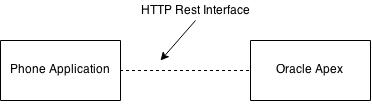
\includegraphics[width=0.5\textwidth]{diagrams/initialblockdiagram}
    \caption{Original design of the application}
    \label{fig:apex_block_diagram_image}
\end{figure} 

\subsubsection*{Functionality}
\label{sec:functionality}

Assessing the functional requirements required breaking down the concept into its core components. Most noticeably posting, viewing and being notified about tags were the core functionality for the application. Without these features the application could not achieve the goals set out in the original specification, thus undermining the usefulness of the finished application.\\
\\
Viewing a message that is left in the application is a core part of the functionality that is required by the application. It should be very easy and uncomplicated for the user to view a tag that has been left by their friends. The application's overall success will most possibly rest on the speed of viewing a message and quickly being able to leave feedback on the tag that has been left. The UI should be easy to interpret with the minimal UI on the screen to ensure that there is no confusion in the message that is trying to be conveyed. A simple and minimal UI also gives the application an attractive aesthetic that should mean that users are attracted to using the application. It should be easy for the user to decide if the tag is publicly available or limited to friends to ensure the flexibility of the application.\\
\\
An equally important feature that makes the application is the posting of messages. Without the ability to post a message the application is a void concept and generally to view messages there needs to be the ability to post messages. Again the key aim of the application is to make it easy to leave messages without any extra complexity that might discourage the user from leaving a message. The UI should be as minimal as possible while portraying the intent of the screen in a simple and straight forward way. Some clever UI design should help draw the interest into the page and enable the user to understand what is happening. The use of a map fragment on this page to show where the user is when they post their message is a good way to draw attention into the posting of a message. The user should be able to enter a message of a reasonable length into the fields within the application.\\
\\
The final core functionality that is integral to get the application to work as desired is the notification portion which notifies the user of the tags that are near by to the user. This should run with no input from the user and should quickly and efficiently provide the user information about the nearby tag. When the user interacts with the notification then they should be able to quickly and effectively navigate to the view message page. They will not have to go into the application itself to select this but the notification will automatically take the user to the view message screen for them to interpret what the message is.\\
\\
More minor functionality is dealing with friends within the application, so adding the user's friends so that they can interact with them within the application. Adding friends to their account should be straightforward with a search that enables them to find and add them to their account. This should also not be a cluttered page with the bare minimum UI elements to get the job done correctly as this should minimise the confusion from using the application and means it should be more likely that users user the application and recommend it on to their friends to actually use it. Continuation of the friends theme is that it should be very easy for users to add viability to messages for their friends to view it. Giving a user viability should mean that they will get notified of the message when they are close by to it.\\
\\
The application will also require having some operations for dealing with authentication with the server. So it is essential for the application to have screens to register and login to these screens should be as simple as possible, only asking the true essentials to get the job done, with clear and simple forms that will not lead to confusion and frustration that would lead to them being put off using the application. Keeping the forms simple should also improve security as it's less fields to protect from attack and thus being compromised by a potential malicious user.

\subsubsection*{UI mock-ups}

Once the application had been broken down into the various functional areas I started to do some rough user interface layouts on paper. Once they were to a satisfactory level they were converted into digital mock-ups using Balsamiq which created the figures \ref{fig:application_home_page_image}, \ref{fig:add_friend_activity_image}, \ref{fig:add_tag_activity_image}, \ref{fig:viewing_message_image}, \ref{fig:giving_friends_visability_image}, \ref{fig:login_activity_image}, \ref{fig:registration_activity_image} and \ref{fig:notification_image}. \\
\\
The UI design takes some inspiration from other phone applications, in particular Snap Chat with the way of quickly sharing messages and Facebook with the quickly accessible stacked menus. The main reason I took inspiration from Snap Chat is because their application is very quick to use and post messages and the general concept of Lo Se Sono is almost the same bar and locations are used rather than pictures and there is no set timeout on the tags.\\
\\
At the time of creating the mock ups it was not clear for which platform the application was going to be implemented, so the designs have remained very generic without being OS specific.\\
\\
These UI mock-ups were used to create the final application. The designs may have been slightly modified between the original design and the final implementation within the application.\\
\\
Figure \ref{fig:application_home_page_image} is the design for the main page of the application and where the users arrive when the application launches, so it is of utmost importance that this page is easy to navigate and informative to the user. The UI has been intentionally designed to show the tags that are most relevant to the user at the time they have opened the application, showing the tags in their immediate vicinity. These can be either the user's own tags or their friends who have left them there.\\

\begin{figure}[H]
    \centering
    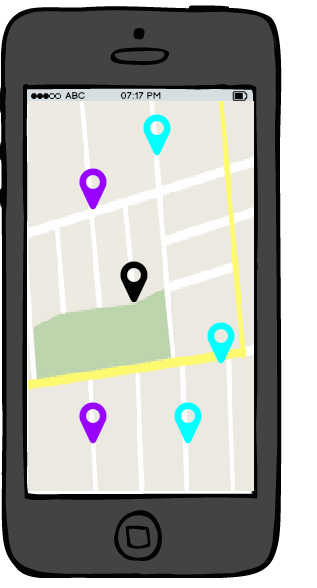
\includegraphics[width=0.25\textwidth]{uimockups/homepage}
    \caption{Application home page}
    \label{fig:application_home_page_image}
\end{figure}

\noindent
In figure \ref{fig:add_tag_activity_image} we are showing the initial design for adding a tag to the map. The key idea is to make it quick and easy to add a tag to the map and make it quickly accessible to the user's friends so they can be promptly notified about the tag their friend has added.\\

\begin{figure}[H]
    \centering
    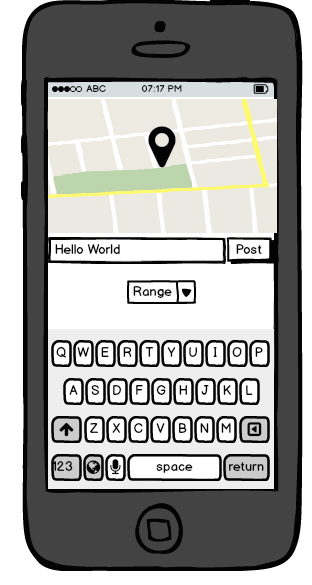
\includegraphics[width=0.25\textwidth]{uimockups/addtag}
    \caption{Adding a tag activity}
    \label{fig:add_tag_activity_image}
\end{figure}

\noindent
Pictured in figure \ref{fig:giving_friends_visability_image} is the screen that enables user's friends to view a message that has been left. It should be relatively straight forward and easy to interpret. The design has changed ever so slightly in the final implementation to try and make it fit in better with the Android design principles.\\

\begin{figure}[H]
    \centering
    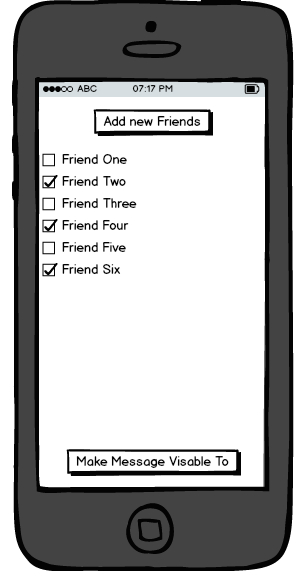
\includegraphics[width=0.25\textwidth]{uimockups/friendsvisability}
    \caption{Giving friends ability to view message}
    \label{fig:giving_friends_visability_image}
\end{figure} 

\noindent
This is the UI in figure \ref{fig:add_friend_activity_image}. To add a new user to the user's friends list it gives the user the ability to search for their friends using their names. In the final version of the application the search functionality remains unfinished within the UI, but was partially completed within the server side application. When this functionality is implemented it should make it very easy for the user to add new friends within the application, thus expanding the audience of the application.\\

\begin{figure}[H]
    \centering
    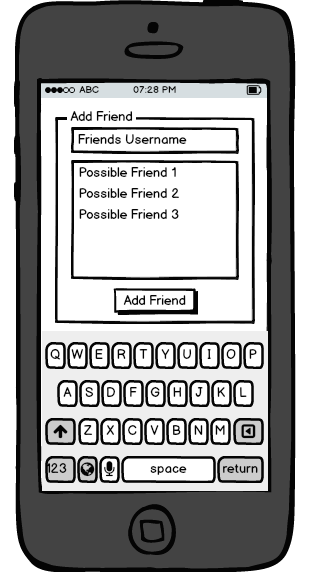
\includegraphics[width=0.25\textwidth]{uimockups/addfriend}
    \caption{Adding Friend activity}
    \label{fig:add_friend_activity_image}
\end{figure} 

\noindent
This figure \ref{fig:viewing_message_image} shows the viewing of a message. This is the screen that has changed the most from the original UI mock ups, where the icons and location of the voting section has been moved to be above the commenting area. There is also now a fixed area at the bottom for adding a comment, along with each comment section now including their own voting sections. But again the changes to the initial designs have intentionally been very minor.\\

\begin{figure}[H]
    \centering
    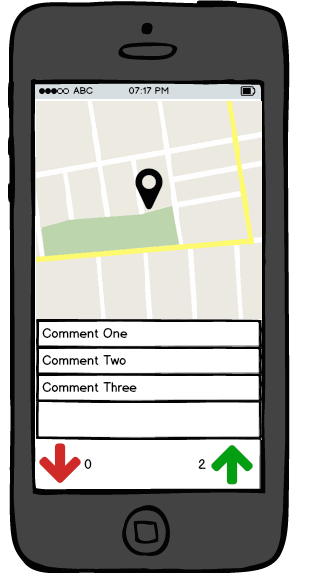
\includegraphics[width=0.25\textwidth]{uimockups/viewmessage}
    \caption{Viewing a message}
    \label{fig:viewing_message_image}
\end{figure} 

\noindent
The image below in figure \ref{fig:login_activity_image} shows the login screen for the application. This was intentionally kept simplistic to ensure that it is easy for the user to interpret and should make it fairly secure against attacks as there are less fields to attack.\\

\begin{figure}[H]
    \centering
    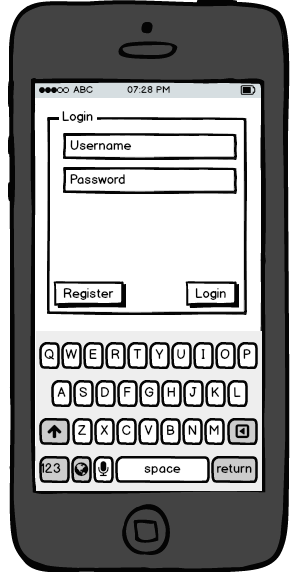
\includegraphics[width=0.25\textwidth]{uimockups/login}
    \caption{Login Activity for the application}
    \label{fig:login_activity_image}
\end{figure} 

\noindent
Screenshot pictured in figure \ref{fig:registration_activity_image} describes the registration page within the application that enables the user to register to use the application. Again it has been kept simple to avoid confusion and ensure that the user can navigate it easily. This should ease annoyance when people are using the application for the first time.\\

\begin{figure}[H]
    \centering
    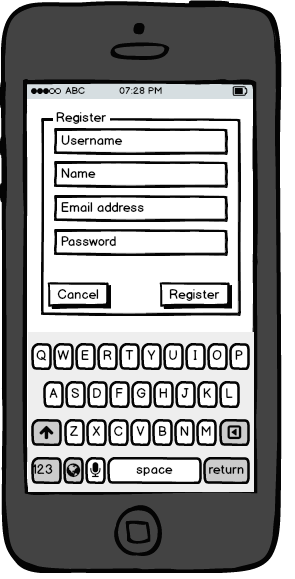
\includegraphics[width=0.25\textwidth]{uimockups/register}
    \caption{This is the activity for registering to use the application}
    \label{fig:registration_activity_image}
\end{figure} 

\noindent
This screenshot in figure \ref{fig:notification_image} is an example notification for the application. In the final application this does not look anything like this due to the fact we are using the Google Android notification API and notifications do not appear in this way.\\

\begin{figure}[H]
    \centering
    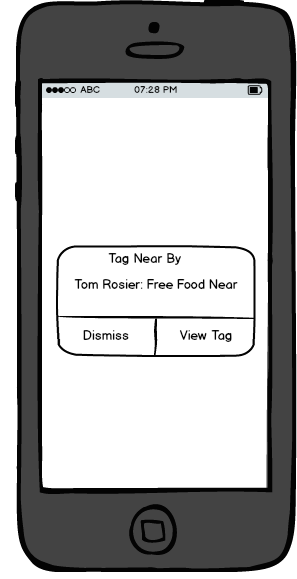
\includegraphics[width=0.25\textwidth]{uimockups/notification}
    \caption{Notification that there is a tag near by}
    \label{fig:notification_image}
\end{figure} 

\noindent
These designs were used as reference to build the applications UI for the final design. They have intentionally kept similar to the original mock-ups as it was felt that the designs would be easy for users to interpret and a good starting point.

\subsection{Final Implementation}

As the project was developed in an eXtream programing style there was not much design done up front. The major design that was done up front was a list of the main functionality within the application and the final implementation of those features were done in an iterative form. There was a very initial block diagram done showing the different main sections of the application, which is shown in figure \ref{fig:initial_diagram_image}. This is the basic design of the application without any of the specifics, e.g not detailing the libraries that have been used to implement the full application.\\

\begin{figure}[H]
    \centering
    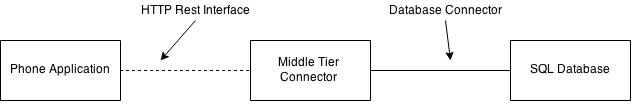
\includegraphics[width=\textwidth]{diagrams/blockdiagram}
    \caption{Very simple block diagram from the start of development}
    \label{fig:initial_diagram_image}
\end{figure} 

\noindent
The final implementation started with spike work into different frameworks that could be used for the development of the project. I started with the Phone side of the application where there was research into whether to use Phone Gapp or to go for a native application. The reasoning and decision to use an exclusively Google Android are covered in section '\ref{sec:android_choice_of_tech} Choice of technologies'.\\
\\
Next the focus moved onto the server side application. The choice of server side environment was focused on looking at cutting edge but also fairly mature server side platforms. The choice was between Node.js with express, Node.js with HAPI.js, Node.js with StrongLoop, Python Flask or Java TomCat. Please refer to '\ref{sec:node_choice_of_tech} Choice of technologies' for more in detail discussion about the rational between the choice of server side frameworks.\\
\\
Finally the decision turned to how the data would be stored within the application. The first decision was between a SQL or NOSQL solution. After some consideration it was decided that even though NOSQL is an interesting new area, it would be best to stick with the skills already learned as taking on too many new frameworks could compromise the success of the project. The final decision was to choose between what type of SQL engine to use to hold and process the data within the application. The decision was between PostgresSQL, My-SQL and SQLite. The pro's and con's are covered in detail in section '\ref{sec:database_choice_of_tech} Choice of technologies'.\\
\\
The diagram in figure \ref{fig:final_block_diagram_image} shows the finished architecture with the joins between each different technology that is needed to make the application work correctly and as desired in the way decided within the functional requirements. It is fairly obvious from the diagram that the application requires a lot of 3rd party libraries to work as intended, heavily relying on the Google Maps API, Android Asynchronous HTTP Client API, HAPI.js \& Sequelize to provide the major components within the project.\\

\begin{figure}[H]
    \centering
    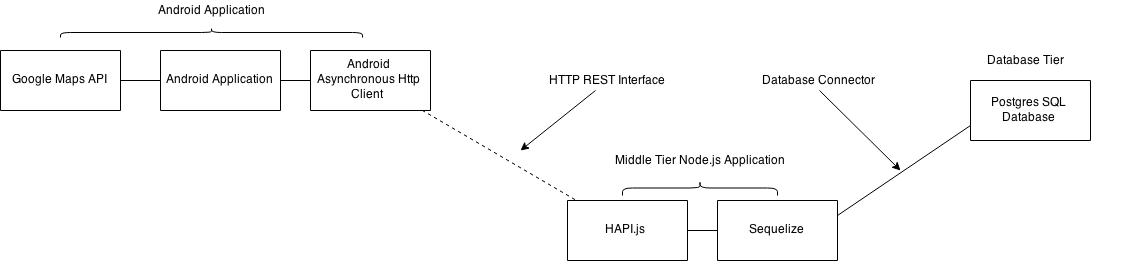
\includegraphics[width=\textwidth]{diagrams/finalblockdiagram}
    \caption{Very simple block diagram of the final architecture}
    \label{fig:final_block_diagram_image}
\end{figure}

\noindent
Standing on the shoulders of giants springs to mind as it would not be possible without all of these 3rd party libraries for the application to work in a usable and robust manner. Even with the use of all these 3rd party libraries there is still a fair bit of custom code to act as an aggregate for all the various parts of the functionality within the project together. The core functionally of the application is complete, but I would currently classify the application as a proof of concept due to the fact the robustness of the application and stability are currently questionable. How these issues will be overcome in the future will be covered in section \ref{sec:development_future_dev}.

\subsection{Future Development}
\label{sec:development_future_dev}

Due to the time constraints and time line of the project it was only possible to complete the application to a proof of concept stage. This section aims to cover the development that would need to take place to make the application viable for release into the consumer space. Firstly the current prototype does not have any consideration taken for preserving power. With the current prototype it very rapidly drains the battery of the devices that it is on and leads to the phone being critically low on battery after a few hours. This will be resolved in further development, which would be more intelligent about when it turns on the GPS, and will use the accelerometers in the phone to gauge if it has moved any considerable distance since the GPS was last turned on and then also changing the duration between the checks to ensure that the phone hasn't moved very often would mean that the duration that we check should decrease, thus helping save the battery on the phone. But in cases where the phone is constantly on the move it is very likely that application will remain very high power due to the nature of GPS. Some effort can be put into the wastage as well if the device can't get a fix, then we should not keep trying as this just drains the battery.\\
\\
Again due to time constraints and how large the catalogue of devices are within Android, there has been limited optimisation of the getting the UI to work perfectly on all devices. Also for the development stage the application has only been designed \& tested on a 1080p device due to being the main device that I had access to, but with more time more consideration and multiple layouts could be made to make the application scale and work correctly on different sized devices.\\
\\
The other point that needs to be raised is due to it being a proof of concept. The application does not fail gracefully and an exception in how the application is used will cause the whole thing to come crashing down around itself without giving any dialog to the user about what has happened. Before the application can be released into the consumer marketplace it will need to have the error catching and handling clearly and robustly implemented so the application can handle any unusual events or unexpected situation. Along with this it is advised to create a full testing suite for the application to ensure that any changes made within the application do not break the whole application and that the operations all complete in the way that they are intended to complete.\\
\\
With theses changes I can see the application being a well used and popular application that will make it an interesting concept that people will pickup and use. I would not consider releasing the application until these changes have been done, as it would not reflect well on the developers to have these issues within the early releases of the code.

\section{Client Side}

%Alison got to here.

The client side part of the application is the part that user actually sees and interacts with, for this project it was elected to use a Google Android phone application to be the main focus for the end user. It needs to act as a way to draw users into using the concept and illustrating the benefits of the ideas behind the application as a whole, it needs to be robust and usable for it to gain wide adoption within the consumer space. If users find the application fun and easy to use it is highly likely they will recommend the application to there friends and it will gain widespread adoption within the popular culture which would be a ideal situation and would mean that project has been successful.

\subsection{Why A Android Application}

Android is a cutting edge mobile platform that is used by many millions of people it is statistically speaking the most popular mobile platform out there with over 50\% market cover \cite{statista:devicestats:2015:online}. To get near blanket market coverage it would be best to develop for Apple iOS as well as it has a market share of over 40\% but due to the time constraints of the project it is only possible to target one of theses platforms, due to have a multitude of Android devices close to hand it only seemed sensible to develop for Android over its competitors, for more detailed explanation of why the choice was to use Android refer to this section \ref{sec:android_choice_of_tech}.\\
\\
Android has is a very diverse selection of devices it will run on, as Google does not limit what devices that it can be run on so any hardware manufacture can decide to create an Android device meaning that they can vary massively between devices there is almost an infinite array of screen sizes and screen resolutions that Android will run on along with a large array of different processors that it will run on due in part to Androids open sourced routes and its deep origins from Linux it gives it a very strong versatility and this means its very popular with the computer science community and users that like to tinker. Although one of the main drawbacks to Android is that ecosystem is fairly fragmented with many different versions of the operating system out in the public domain which means its difficult to get applications developed on Android to work on all of the devices out in the public domain either due to there form factors or due to the fact they are running a out dated version of the operating system which leads to incomparability with the newer code libraries. Luckily 93\% of devices \cite{google:osstats:2015:online} out in the wild are running fairly recent versions with the majority of theses devices running a API level between 15 and 22 which means that most code will run on the majority of devices as long as the developer is not seeking the most bleeding edge API's for there application.\\
\\
For this project it was decided to target the application at API level 14 which is known as 'Ice Cream Sandwich' and higher as this would give the ability to use fairly recent API's but also covering the mass majority of the devices out in the wild. API level 14 dates back to 2011 with the launch of Android 4.0 which means that we can support nearly all devices that were released in the last 5 years as flag ship phones from 2009 \& 2010 are fairly likely to still receive updates to 'Ice Create Sandwich'. Due to the user community that goes with Android it is fairly likely that theses old devices will have been updated via 3rd parties to run newer versions of Android than the original manufactures intended.\\
\\
The Android developers hub provides a very comprehensive set of API documentation along with tutorials on how to develop for Android with best practice documentation on the best way to design the application to make it fit in with the style of the Android ecosystem, some of the early research done for the project was based on reading the Android material design manual to ensure the application had a consistent theme and would be accessible to all sorts of different devices and users which would ultimately help with the adoption and usability of the final application.

\subsection{Choice of Technologies}
\label{sec:android_choice_of_tech}

The spike work / research that was carried out in the design stage started out by reading about the development experiences of various teams Phone Gapp vs Native to develop there various phone application and the reviews that I got seemed to be very mixed they ranged from saying to avoid or this is the best thing ever, with no clear way to move forward it the next stage was to research the API's that would be essential to the application working this being the Mapping API's and the GPS location. It quickly came apparent although Phone Gapp its fairly mature it could not compare to the libraries that were offered by the native solution.\\
\\
One of the benefits of using Phone Gapp over native is that it uses standard web technologies for example HTML, JavaScript \& CSS which I as the developer already knew fairly well and would not need to learn a new language to work on the application but this would still require learning a new framework to work on the application. Another benefit of using Phone Gapp is that the application will run on a multitude of devices from Apple iOS, Google Android and Microsoft Windows Phone where as choosing to go native means that application will only work on the framework and device it is programmed for.\\
\\
One of the major downsides of using Phone Gapp is that if there is not a library that exists for a given problem within the application then the developer is required to write in native code a library to couple the Phone Gapp application to the function provided by the phone. Due to this it was decided it would be best to just develop the application in native code as it eliminates theses coupling issues if they do arise. Along with the extra performance given by running within the native framework and not having another interpretive layer between the user and the phones hardware gives the developer and ultimately a better experience with the application.\\
\\
It was clear the best way forward was to use native development, my choice was then limited by what hardware that I already owned and due to only owning a Android based phone the decision was essentially made up for me and thus the development of a native Android application was the way forward, the major downside of developing for Android that although it is the majority platform out there, Android users tend to be less engaged with the application community than iOS users meaning that the adoption would be potentially hurt by deciding to target Android first. In the commercial work it is very likely that developers will create a native application for both Android and iOS to make sure there is adoption on the two main smart device platforms thus leading to near blanket coverage of the market.\\
\\
For the choice in Mapping API's there was only two solutions using official Google Maps API or Nutiteq Maps SDK, after some consideration it was apparent that Nutiteq was not as mature or well supported as the official Google Maps but did offer some nice additional features that the Google Maps API did not like the ability to have offline maps and the use of custom perspectives. It was decided to use the Google Mapping API as it had a mature community and is well supported, but if the decision was made at the end of the project the use of the Nutiteq API may have been a better choice due to the very limited and outdated documentation for the Google API which was a big disappointment.\\
\\
For dealing with rest requests it was decided to use Asynchronous HTTP Client for Android \cite{nknj:AndroidAsynchronousHttpClientloopjandthePersistentCookieStore:2013:online} as this was a well documented API with all the functionality that was needed to deal with all of the requests that needed to be carried out within the application, it gives a good flexibility for processing JSON objects that are returned from the server along with doing it all asynchronously to which will improve the snappiness of the application while dealing with requests.\\
\\
The interaction between the server and the Android Application is provided by an HTTP RESTful interface which enables robust and reliable standard for sending transmitting data, the ability to send JSON objects directly back and forth between the server and client makes data manipulation easy and means that the interface between the client and server is not platform or language specific which means it should be easy to add in another client that can use the API provided by for the application.

\subsection{Initial Design}

As mentioned previously the application was developed in a evolutionary way, with functionality only being added when it was essential to proceed with the application this mean there was not much in the way of up front design. For the Android side of the application the the way in upfront of design was to create a list of the functional requirements of the application detailing what the application needed to achieve to be a successful project these theses are listed within section \ref{sec:global_initial_design} and was mostly orientated towards the UI design of the application rather than the background architecture the architecture will be covered in detail in section \ref{sec:android_application_structure}.\\
\\
In the early thoughts about the layout and design of the application it was apparent that a model view controller approach should be taken to the design of each parts of the application, meaning that data structures, and viewing of the data are segregated out and there is a interconnecting layer between them to create a structure that is decoupled meaning that code is not written specifically to do one job and can be reused in many places to do many jobs which simplifies duplicated code and should ensure that code only has to be debugged in one place and is not copied to multiple locations throughout the application which should ensure that bugs are not encroached into the code base which could compromise the robustness of the application as a whole.\\
\\
Most of the initial design for the application was to investigate the frameworks that would be used within the application ensuring that they would suite the functionality requirements for the application, at first it was fairly hard to find a well documented and robust framework for dealing with HTTP requests to the background services to get the information that will be displayed within the application. The first framework that was tried seemed to have some stability issues and deal with all requests synchronously which mean the application would stutter while trying to retrieve data along with having stability issues which made the application unstable in real world operations. Another chunk of the early design stage was trying to get the Google Maps API to respond in a way that was usable for the needs of the project, which included the ability to tag locations and show robust labeling with the custom messages left by the user.

\subsection{Application Structure}
\label{sec:android_application_structure}

The structure of the application is based around it activities which is Android's name for screens, each activity has its own job to fill a place within the functional requirements of the application theses requirements can be found in section \ref{sec:functionality}. Usually it is a activity for each of the function so for example creating a new tag would have its own activity with its own supporting classes. An example of how the code is structured for each of the activities can be seen in figure \ref{fig:activity_interation_image}, data flows two and from the screens back and forth to the rest client part of the application that deals with interaction with the server either retrieving or sending data back to enable the functionality within the application.\\

\begin{figure}[H]
    \centering
    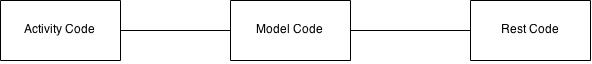
\includegraphics[width=\textwidth]{diagrams/activityinteraction}
    \caption{This is the simplified interaction between activities}
    \label{fig:activity_interation_image}
\end{figure} 

\noindent
Model and RESTful client layers of the structure are shared between larger parts of the functionality and may encapsulate everything to do with for example sending and receiving messages, along with all the other permutation of this format being contained within the same class to group them together functionality and make them easy to access and work with. They have tried to be kept as uniform and repetition kept to a bare minimum which should help with creating a easy to work on easy to maintain application that is an enjoyable code base to work on.\\
\\
The main point of entry for the application is the Navigation Activity which is the screen that shows all of the tags that are close by to the current user and there relevant to them, all of the application is ran from this point from this screen it is possible to reach all of the other activities and is the home page that the users land on when the execution begins it is the focal point of the application and is a return point after every operation has finished.\\
\\
There are other services that are run along side the activities one example of this is the notification service that enables the user to receive notifications that are relevant to them without viewing the application, they are push notifications the end user can view outside of the application and they add an extra bit to the user experience of the application.

\subsection{Caveats}

This section is dedicated to some of the shortcoming in the design of the Android Application and explanation of the issues. As Fred Brooks said in the Mythical Man Month \cite{fredbrooks:throwoneaway:1995:online} "Plan to throw one away; you will anyway" and it is fairly true in this situation, developing a application in a totally new framework to the developer means that some of the design choices can be misguided which results in the applications overall stability and design being hurt. Overall the design of the application as a whole is not bad but there are places where it is a little patchy and not designed to the best standard.\\
\\
The application will need some refactoring and design tweaking to make it a rewarding code base to work on as it stands if more functionality was added to some of the activities it would quickly become very difficult to work on with Spagetti code being the only way forward to patch on the new functionality. This will ultimately lead to a bad customer experience which will alienate users of the application and make them not want to use the application which would kill any representation that the application gains.\\
\\
As mentioned previously the fact that the application is only available for Android means that the audience for the application is limited to only half of the potential users out in the world due to the other users using Apple iOS, As part of the further development of the application it would be advised to develop an Apple iOS version of the application or scrap the current code base and move to Phone Gapp based application which would mean the application will work on any of the major smart phone operating systems.\\
\\
More research could of been done in implementing the various background services that are used within the application as they are in the version included with this a bit temperamental, this is somewhat down to the very limited documentation offered by Google on how to implement features that have provided by the Android Operating System its self. This was also not aided by the fact that some of the documentation for the various API's most notably the Google Maps API is heavily out of date and will not actually work on the device with the instructions given in the API documentation.

\section{Server Side}

The server side of the application is the part of the user does not directly interact with and handles the underlying functions behind the application working correctly this functionality gives an underlying service that enables the usability of the application. Theses services are responsible for supporting the RESTful interface between the application and back end, along with providing coupling between the RESTful interface and the database.\\
\\
The back end services are there to provide an effective data store for the users information along with providing the layer to create the interaction between users as the data is stored and processed on the server verses all the information being stored on the clients devices which would lead to the application being unmanageable due to data being placed in multiple different places along with when a device is offline then the data is unaccessible to other users.\\

\subsection{Middle Tier}

The middle tier is the connective tissue of the application acting as a intermediary between the database and the front end application. Its main purpose is to act as a HTTP server along with a client authentication point to ensure that only registered users can use the application. It is connected to a PostgresSQL database which handles storing data in a persistent form which can be easily interacted and manipulated to archive the desired functionality within the application that the end user can see and gives the application the desired effect.\\
\\
For this important task it was decided to use enterprise level frameworks and technologies, it was integral that the platform and the frameworks that were used to provide the functionality were robust, flexible and easy to work with I concluded to use Node.js \cite{nodeteam:node:2015:online} with the HAPI.js \cite{hapiteam:hapti:2015:online} was the best route to go down as it is fairly cutting edge but also has big supporters and a good support community, HAPI.js provided a robust and usable framework that was not overly complicated for the scenario that it would be used. It was also felt that the platform that the system is run on is not platform specific and can be run on any of the three main operating systems, thus the background services although have not been tested theoretically will run on a Linux Server along with an Apple OSX Server and Windows Server which means that if a platform change was needed in the future it should be easily possible to move the application's backend over to a different platform. More in depth reasons to why theses platforms / frameworks were chosen can be found in \ref{sec:node_choice_of_tech}.\\
\\
The user of a HTTP RESTful interface between the middle tier and the Android application seemed the most modern and best way of providing an link between the client and the background API that handles the data for the users of the application, it is also not platform specific which means it should be possible to add in other platforms that use the service at later points which can make use of the platform that already exists. This also translates over to the backend of the application because if the backend was ever replaced with another platform and services as long as the API end points returned the same data and the authentication worked in the same way then any client side application will work in the same way and the users would not see any different in the service.\\
\\
For the design of the backend application it was key to make it as modular as possible to ensure that it is fairly easy to add new functionality in as it was decided it would be best to use dynamic loading where possible, the application takes a list of route files which are for each part of the functionality given for the application for example there may be a route dedicated to all things messaging and if there was a need for a new bit of functionality not seen at the start of development then another route can be loaded in to add functionality needed within the backend application to handle the new functional requirement without the need to redesign the whole application and potentially damage the integrate of the application.\\
\\
Initial design for the backend of the application was to create a list of the corresponding RESTful endpoints for the functionality provided by the Android application, as the project progressed some alterations were made to this initial list for unforeseen functionality changes for example segregating the users messages from the friends messages and not have them all in one rest endpoint.\\
\\
The backend is linked to the database through a database connector the one that has been used is called Sequelize \cite{SaschaDepold:Sequelize:2015:online} and provides a Object Relational Mapping(ORM) which was originally going to be used within the application but it was quickly decided to use the raw SQL functions provided by the connector. The ORM functionality may be implemented properly at some point in the future development of the application and it was personal preference to elect to use the raw SQL interface as it was what I was more comfortable with and allowed better control over the data that was being returned from the database. Sequelize had one very nice feature that meant that JSON objects could be returned directly from the database which in some cases can be sent straight to the front end application without modification, which helps reduce the complexity within the application as a whole and makes it easier to debug in the long run.

\subsubsection*{Choice of Technologies}
\label{sec:node_choice_of_tech}

There were many different choices that could of been made for the platform and framework to run the back end application on, the 4 major platforms that it came to decide from was Java, PHP, Python and Node.js. Java was quickly ruled out as it was felt that it was to heavy weight and clunky for the application although it would be a better choice if the application became a heavy weight enterprise level application, Oracle offer very good support for Java based applications with very comprehensive API documentation along with the fact that the Android Side is developed in Java meaning there would only be one programming language for the whole project reducing the learning for the project as a whole but it was felt it would not be a good fit for the project. Next the attention was turned to PHP, PHP is a well known language for doing web based API's and is a long standing contender for doing this type of work my prior experience of PHP had not been very rewarding experience and it was a horrible language to work with which instantly gave me concerns to where it stands within this project along with some reports floating around at the time of starting the project about serious security issues PHP was dead in the water.\\
\\
This is where things get a bit more interesting the choice between Python and Node.js was very close due to the fact that they are up coming platforms with strong enterprise level functions along with being very powerful dynamically typed languages which enables high flexibility with how the application is designed. Both of the platform have very good frameworks to enable robust and clever web frameworks which would be perfect for this project along with very mature automated installation tools for the extra libraries that would be needed to run the software with Pythons PIP and Node.js's NPM tools making the portability of the applications much better solution than the PHP and Java alternatives. Ultimately the choice between the two platforms was made on what I as the developer already knew Python nearly won the battle but due to already knowing Node.js and the fact I would have to relearn Java and Android it was decided that learning 2 new languages may be a tall order and would be likely enough to jeopardise the project as a whole this was not a risk that I wanted to take.\\
\\
After deciding that Node.js was the way forward the next major decision was to choose what framework to use to build up the web services there was quite a few choices for this Express.js, Restify, HAPI.js and StrongLoop. Some of the reasoning came from the blog post by Alex Gorbatchev \cite{AlexGorbatchev:CompairingExpressRestifyHapLoopBack:2015:online} but I felt it was a little bit skewed by the fact it looked like he was a developer for StrongLoop along with the page being hosted on there blog. Restify was the first to be looked at as it promised the ease of creating simple restful services and strongly advertised it was intended for API's rather than websites, but after some close investigation it was felt that it was to restrictive and didn't have much support from large organisations and looking closer into support there did not seem to have a large community behind it. Next the attention was turned to Express.js which on the surface looked like it would most likely be the framework choosen for the application I had previously used Express.js and had enjoyed working with it, it is also robust, well tested, well proven but the only negative that can be said about it is that it is aimed more towards browser based web applications which is not what is desired for the project I am 100\% sure that Express.js could of been the de facto framework used within the project but I felt like a challenge and wanted to use something new.\\
\\
Next we will talk about the two frameworks that were in the top two, after throwing out Express.js my attention was drawn to StrongLoop after browsing there API documentation and marveling how clean and pretty the code looked I was pretty set on using it, I setup a development environment for the framework and immediately hit a brick wall with the learning curb presented by StrongLoop. StrongLoop is a Model View Control(MVC) based framework and requires lots of configuration to work correctly and relies on Object Relation Mapping to interact with its database. After couple days of going know-where it was best to reassess the decision after finding that the strict MVC to restrictive getting in the way of getting work actually completed the conclusion was to re-investigate the option at this point HAPI.js popped up as an option after further some investigation. HAPI.js seemed to have everything going for it it had big name supporters Disney, Yahoo, PayPal, Mozilla and Walmart just to name a few along with a strong development community and very useful Internet Relay Chat channel that could be used when extra support was needed. With some small spike work it was clear to see that HAPI.js with its simple but very powerful API was the way forward, within a few hours the progress with HAPI.js was impressive and with many examples and extra that can be used to speed up development it was the right decision for this project.

\subsubsection*{RESTful interface}

The RESTful interface provides communication between the front end application and the backend services, they should be able to carry out all of the functions that are important to the application for filling the functional requirements. RESTful services provide an uniform interface between applications over the HTTP protocol and use standardised HTTP request types for example POST and GET. As it is reasonably likely that the application will be turned into a web application at a later point it was desirable that only POST and GET methods were used to post information back and forth as theses are the only two requests that are allowed by most web browsers, this will ease porting the application to a web application at the later point.\\
\\
The diagram in figure \ref{fig:rest_pai_diagram_image} gives an explanation of all the RESTful end points and there request types that are needed to carry out the operation that is intended of them. The POST options will have extra parameters passed within the HTTP request that will be important to the functionality of the application. 

\begin{figure}[H]
    \centering
    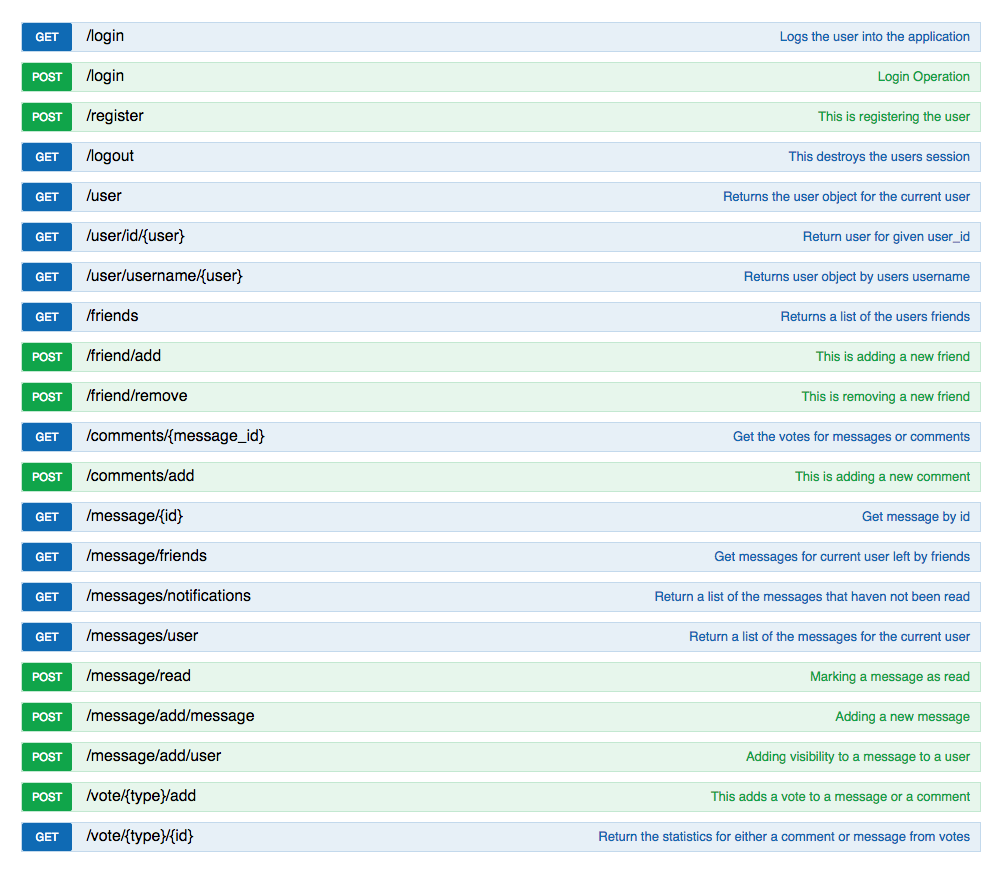
\includegraphics[width=\textwidth]{diagrams/restinterface}
    \caption{These are the endpoints for the REST API}
    \label{fig:rest_pai_diagram_image}
\end{figure} 

\subsubsection*{Structure of application}

The structure of the application is detailed within figure \ref{fig:middle_tier_code}, it has a very simple structure for the main part of the application comprising of the main deployment layer that is statically loaded code which sets up the configuration for the database \& HAPI.js server, the objects that support them are then passed to the route loader that loads the routes code dynamically that allow the application to perform its functional requirements.\\
\\
Each of the dynamically loaded modules is passed the shared object contains the references to the HAPI.js server object and to the database connector, which makes them easily accessible within the dynamically loaded code, each of the routes that are loaded dynamically loaded has its own database connector to enable a somewhat like Model View Controller type of approach to how the classes are structured, the route can call the database connector directly to get the information that is related to its various RESTful API end points that the route services. It has been on purposely done this way to ensure that to ensure flexibility within the application and enable the application to be easily extended without the need to change the main structure of the application to make the new functionality work.\\
\\
More critical parts of the application are statically loaded for example the code that deals with authenticating the user is statically loaded at the begging of authentication to ensure that it is robust and cant be tamped with once it has been loaded. For authentication it is felt that it should be a core part of the design and should be taken with up most respect and should be reasonably well engineered to ensure that the security of the application is not compromised.
 
\begin{figure}[H]
    \centering
    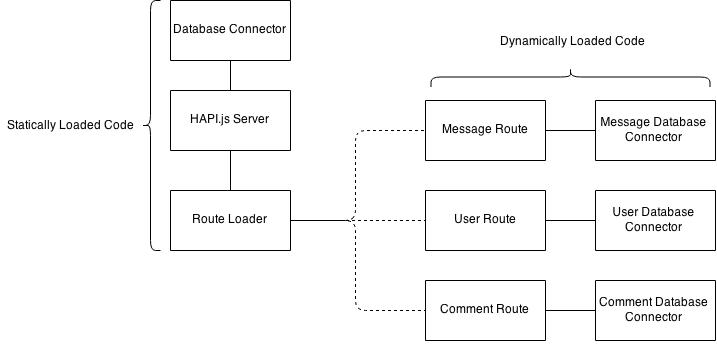
\includegraphics[width=\textwidth]{diagrams/middletier}
    \caption{Detailed structure of middle tier code}
    \label{fig:middle_tier_code}
\end{figure} 

\subsubsection*{Authentication}

The authentication procedure for the application is to used a mixed approach to authenticating the user to use the application, the user must first authenticate them selfs with basic authentication to the server which creates a session for the user and returns a cookie to them, from here the user must the cookie to authenticate them selfs against the API. HAPI.js's handles most of the background tasks for the authentication using some extra modules HAPI-Auth-Basic \& HAPI-Auth-Cookie the hook into the standard configuration to give the extra functionality that is needed for the authentication services, the code that authenticates the users is spread between the HAPI.js application and the database and has been linked together by my own development. More details about the database side of the authentication can be found in section \ref{sec:database_security}.\\
\\
This way of authenticating the user will replaced in the further development that will take place with a better standard for securing the user the use of oauth would be a much more desirable way of authenticating the user to use the middle tier services that the current method of authenticating them, at the time it was implemented into the project the current security was only there as a temporary measure for making the development secure and if time constrains had not be so tight the authentication procedure would of been upgraded to use oauth and a full review of the security procedures would be taken.

\subsection{Database level}

The database level of the application is responsible for creating a persistent store for the data that is created by the users, and making it easy to create links between the data that has been stored. In essence the database does most of the work for the application linking the various data sources together and processing it to give the application all of the its functionality that is needed to make the application work in the way specified by the functional requirements.\\
\\
It is much more efficient to get the database to process the data rather than making the middle tier do the processing work, database engines are very good at processing large amounts of data and creating links between the different types of data that are stored within the database. A database is perfect for storing large amounts of data that needs to be processed quickly and efficiently.\\
\\
It was decided that a SQL based database would be the best way of keeping and linking data together quickly efficiently behind the scenes to give the application the robust and enterprise level feel that is needed for managing and storing data. One of the more advanced features of a database is to allow robust contains to be applied to the data and ensure the data is valid for use within the application.

\subsubsection*{Choice of Technologies}
\label{sec:database_choice_of_tech}
 
It was quite straight forward decision to decide that a SQL based database was the best way forward due to its flexibility and I as a developer have a strong prior knowledge of SQL database's from working for one of the leading database experts Oracle. This was weighed up with learning a new technology the other possible choice was to go with a noSQL type database but due to the complexity of the project it was best to stick with a technology that was already known. Most of the comparison for deciding which platform to use came from Digital Oceans blog post on comparing relational database management systems \ref{ostezer:sqlframeworks:2014:online}.\\
\\
The next decision was to decide what database platform the application would be developed on there was a couple of choices for this MySQL, SQLite and PostgeSQL. SQLite was disregarded very quickly in the investigations as it is meant for much more simplistic applications and would only server an application with a max of 300 users before it would not be able to scale correctly, this is mostly down to the fact that SQLite is intended to be very simple to implement so that it can be used within embedded situations, its main benefit over the other databases is that it is highly portable and does not require large configuration to get it working correctly and would be something that could be a possible to use for caching requests on the client side application to help speed up the Android application.\\
\\
MySQL was the next on the list of platforms to research this would seem a good choice for a small to medium sized project with plenty of flexibility, it gives more advanced features than SQLite with the ability to create database functions to carry out more complicated of tasks, it offers high security features unlike SQLite as it is a custom solution it is highly customisable and can be adapted to work for any given job. Downsides is that it is not fully compliant to the SQL standard it is also missing some more advanced features that are offered by other database engines.\\
\\
The final option that was consider is PostgreSQL it offers a very advanced database engine with advanced features not offered by the other offerings and its main goal is to be standards compliant, it is well known for its data integrity capabilities. PostgresSQL is known for working well with large designs and has better integration than other solutions and rivals some propriety solutions on this matter. Some of the downsides of using PostgreSQL is that it is not very portable it is hard to configure and setup correctly along with being difficult to replicate without spending alot of time ensuring that everything is the same between the two different databases. It also has slower performance compared to some of the other solutions mentioned previously as it is not optimised for exclusively read operations from the database like for example SQLite.\\
\\
Some of the reasons PostgreSQL was chosen for this project were the advanced security features that are offered within expansions, the mature and flexible database functions offered. Probably the most important was the ability to dynamically import JSON objects directly into the database which should simplify working with the RESTful API that we are using within the middle tier as the objects that deals with specifically are all JSON objects and being to directly inject them into the database without manipulation is a very useful feature. 

\subsubsection*{Database structure}

The structure of the database has been designed around the types of data that needed to be stored for the functional requirements of the application to be for filled, the origin of the design was to store the information of the users in a secure and effective manor the focus then moved to on how messages would be stored will all the relevant fields.\\
\\
Next the biggest priority was to ensure that the messages were viewable by the persons friends so the friends section of the database was developed, after this all the auxiliary parts of the application were added this includes the comments and voting sections of the database. The design of the database grew evolutionary style to ensure that all parts were covered for the most part the design was done upfront and then morphed as the development continued.\\
\\
The figure \ref{fig:diagram_database_image} shows the connections between all of the classes and the fields held within each table, looking at this diagram it would appear that user\_id is a very commonly used field within the database which may cause issues in the future as the users table will be the table that will take the most number of requests and this data may need to be de-centralised at some point in the future as it may become a bottleneck in future, intelligent use of indexing and caching may help to prevent issues with this though. One shortcomming in the current design is there no way for there to be pending friends request for users so they will automatically come friends at the current moment the second a request is sent.

\begin{figure}[H]
    \centering
    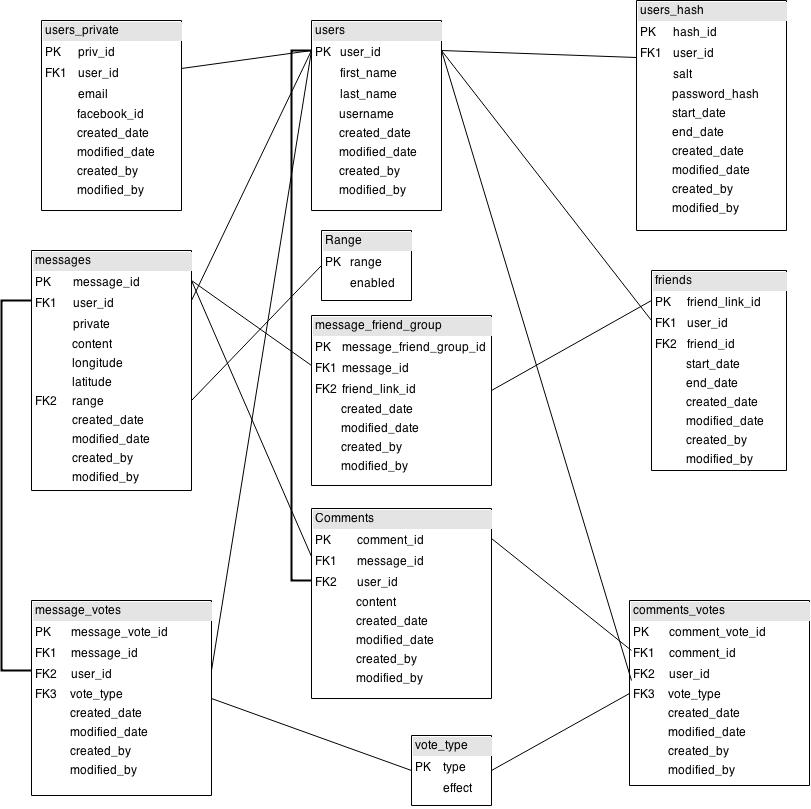
\includegraphics[width=\textwidth]{diagrams/database}
    \caption{This is the database design for the application}
    \label{fig:diagram_database_image}
\end{figure} 

\subsubsection*{Alterations}

The design had to be modified during the implementation of the project, it was mostly to ensure that the database contained all of the relevant data needed to for fill the functional requirements of the project, A later addition to the design was the ability to vote and add comments to messages. The constraints on the tables were added as the project proceeded to ensure that only correct data was entered into the database.\\
\\
One further alteration that will need to be made before the database can be used within a production environment is to add in indexing for the most important columns within the application, indexing them should help improve the performance of the database and ensure than most regularly accessed data is easy to access and is quickly indexed.\\
\\
There will need to be the ability to audit the data as well and this will also be added before the application goes into a full production, this should ensure if there are any issues then they can be traced to where it originates.

\subsubsection*{Protecting secrets}
\label{sec:database_security}

There has careful consideration taken to how sensitive data is stored within the database, the most primitive of the steps taken to help protect the users data was to separate the users data into levels of sensitivity, with the users email address and social media account id's stored away in a separate table to the main users details and there password hashes also kept in a completely different table to the rest of the users data.\\
\\
All actions to do with the users password is processed by the database engine its self, the functions that process to ensure the password is valid are kept within the database and return a status back to the middle tier to tell that the users credentials are valid so there is no chance of of sensitive data being leaked into the middle tier application.\\
\\
The users password is not stored in anyway, a MD5 of the users password is encrypted with an random encryption key which is stored along side the password this should help prevent rainbow attacks on the data left within the database and adds a extra layer of security against the possibility of compromising the data contained within the database.\\
\\
When the application is placed into the public domain steps will be made to improve the security of the data to ensure that no sensitive user data is leaked into the logs or the public domain. Currently the application uses a mixture of blowfish and MD5 to generate the salt and encryption keys that are used to protect the secrets in the application, the use of SHA-2 would be a much better hashing algorithm to use to protect the users data and will be reviewed and implemented in further development.


\chapter{Implementation}

\section{Tools used}

\subsection*{Sublime Text}

\begin{figure}[h]
    \centering
    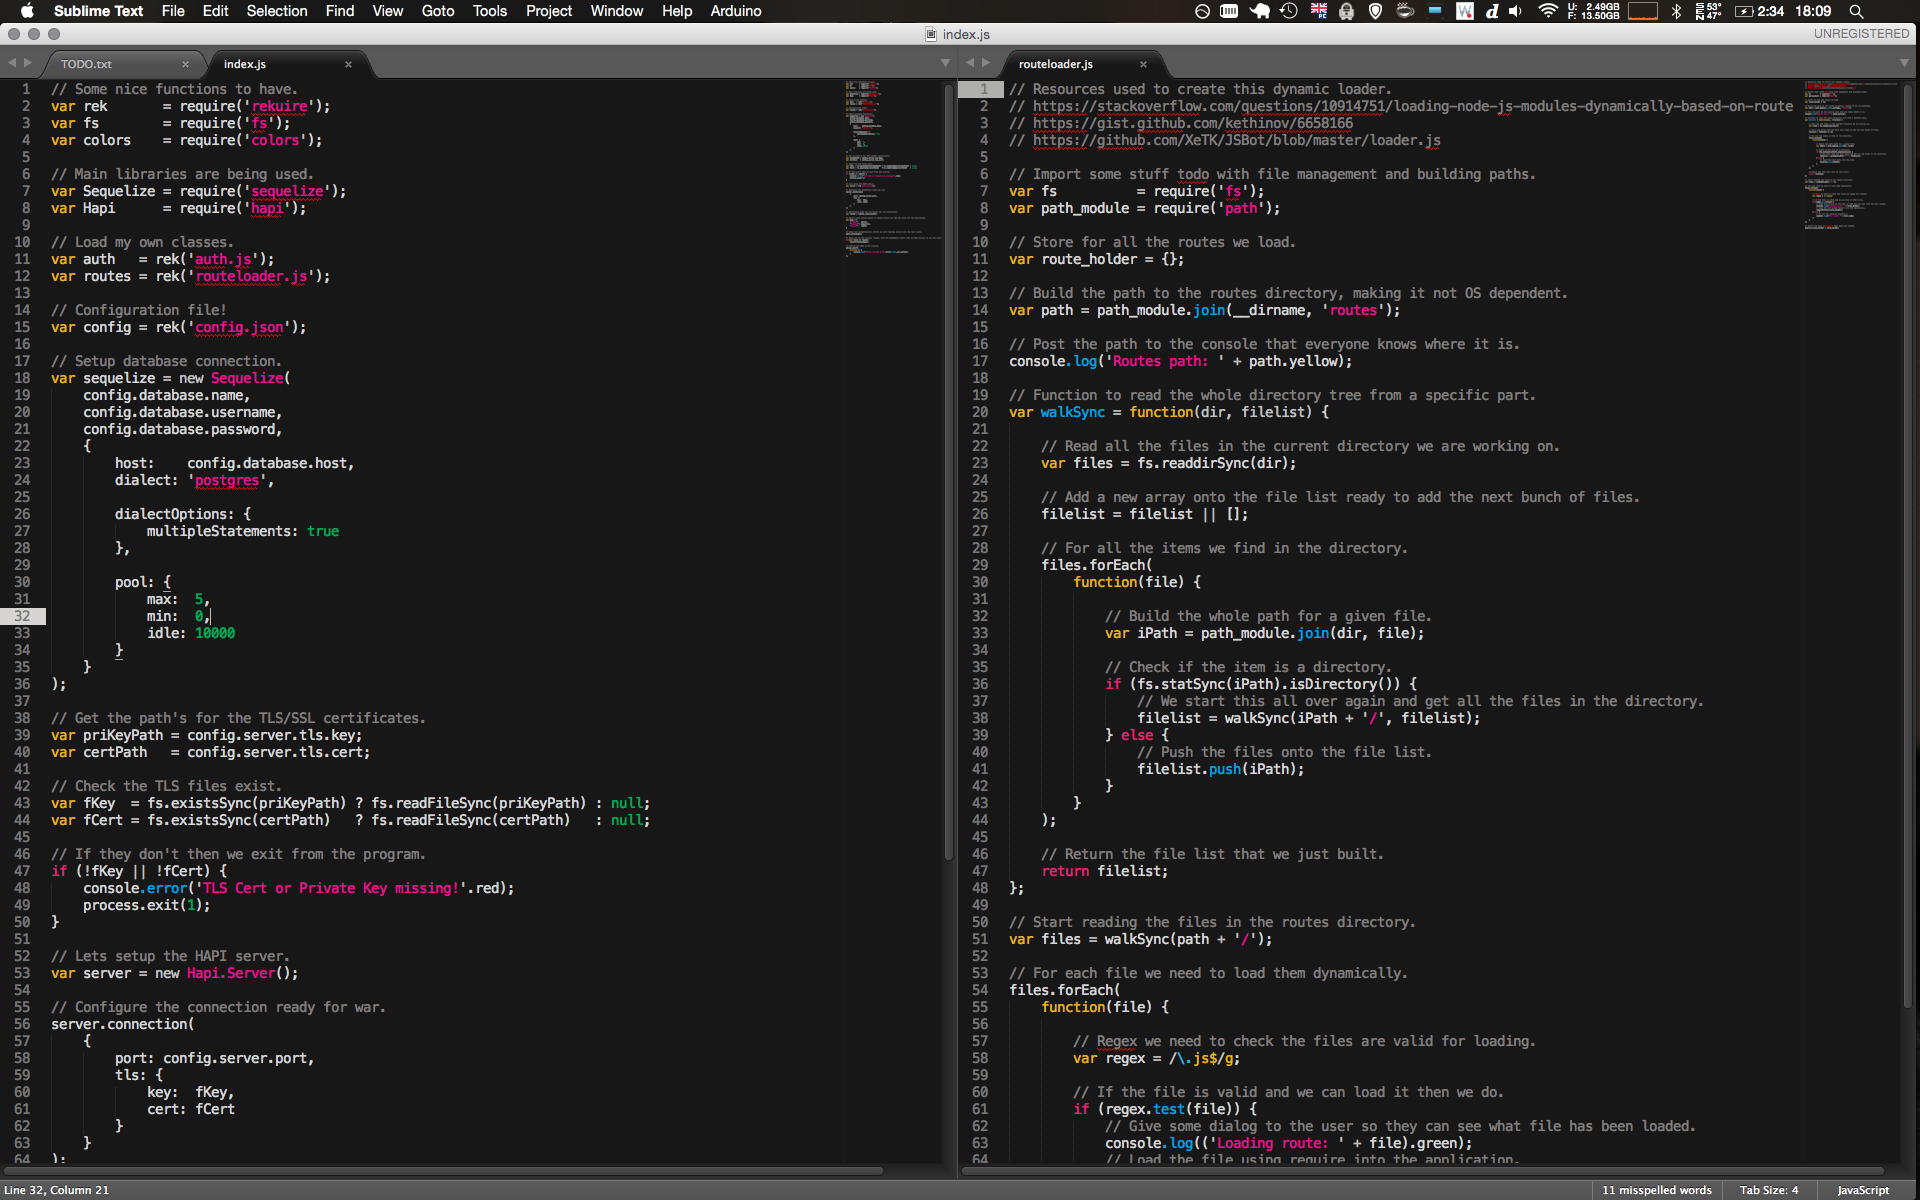
\includegraphics[width=\textwidth]{tools/sublime}
    \caption{Sublime Text 3.0}
    \label{fig:sublime_text_image}
\end{figure} 
\noindent

\subsection*{Android Studio}

\begin{figure}[h]
    \centering
    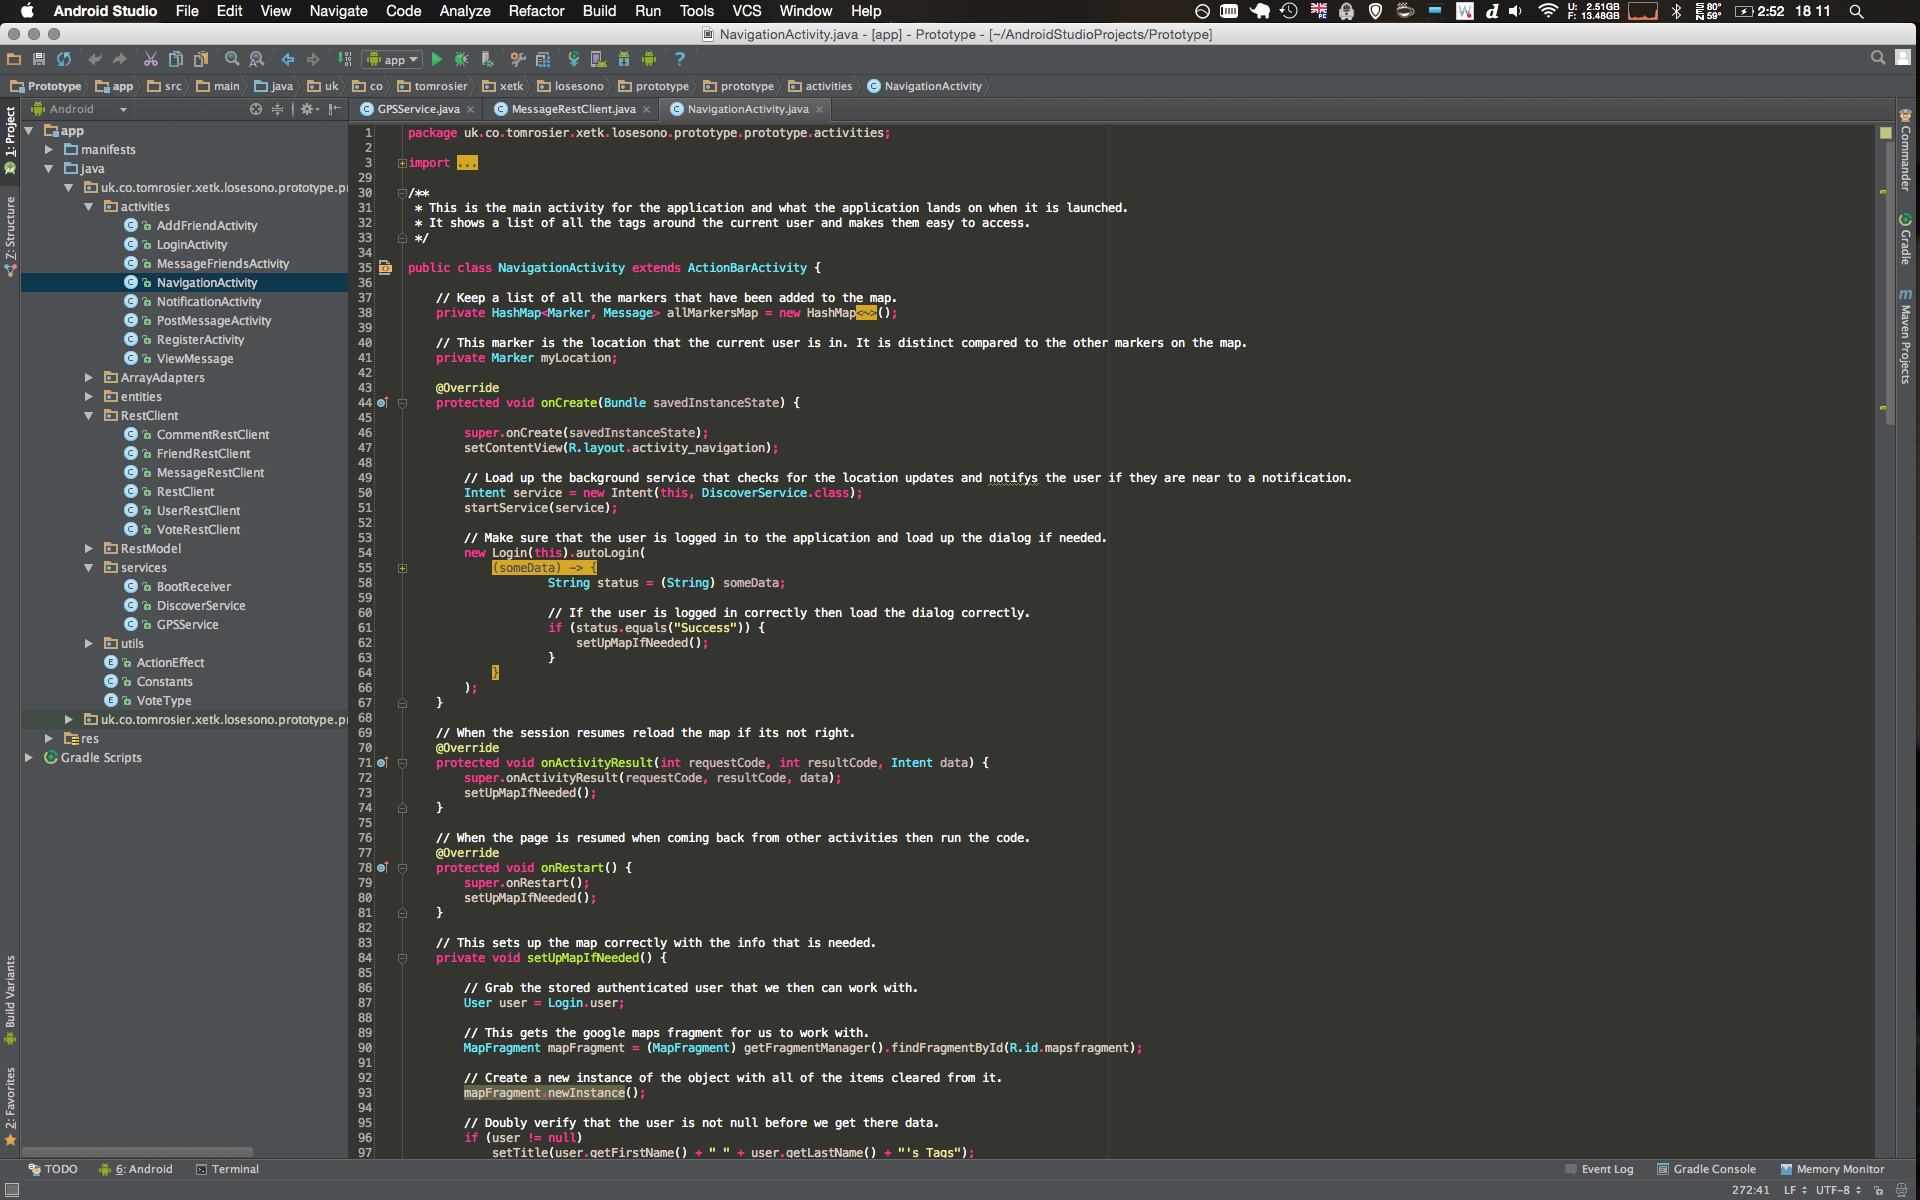
\includegraphics[width=\textwidth]{tools/androidstudio}
    \caption{Android Studio 1.1.0}
    \label{fig:android_studio_image}
\end{figure} 
\noindent

\subsection*{PGAdmin3}

\begin{figure}[h]
    \centering
    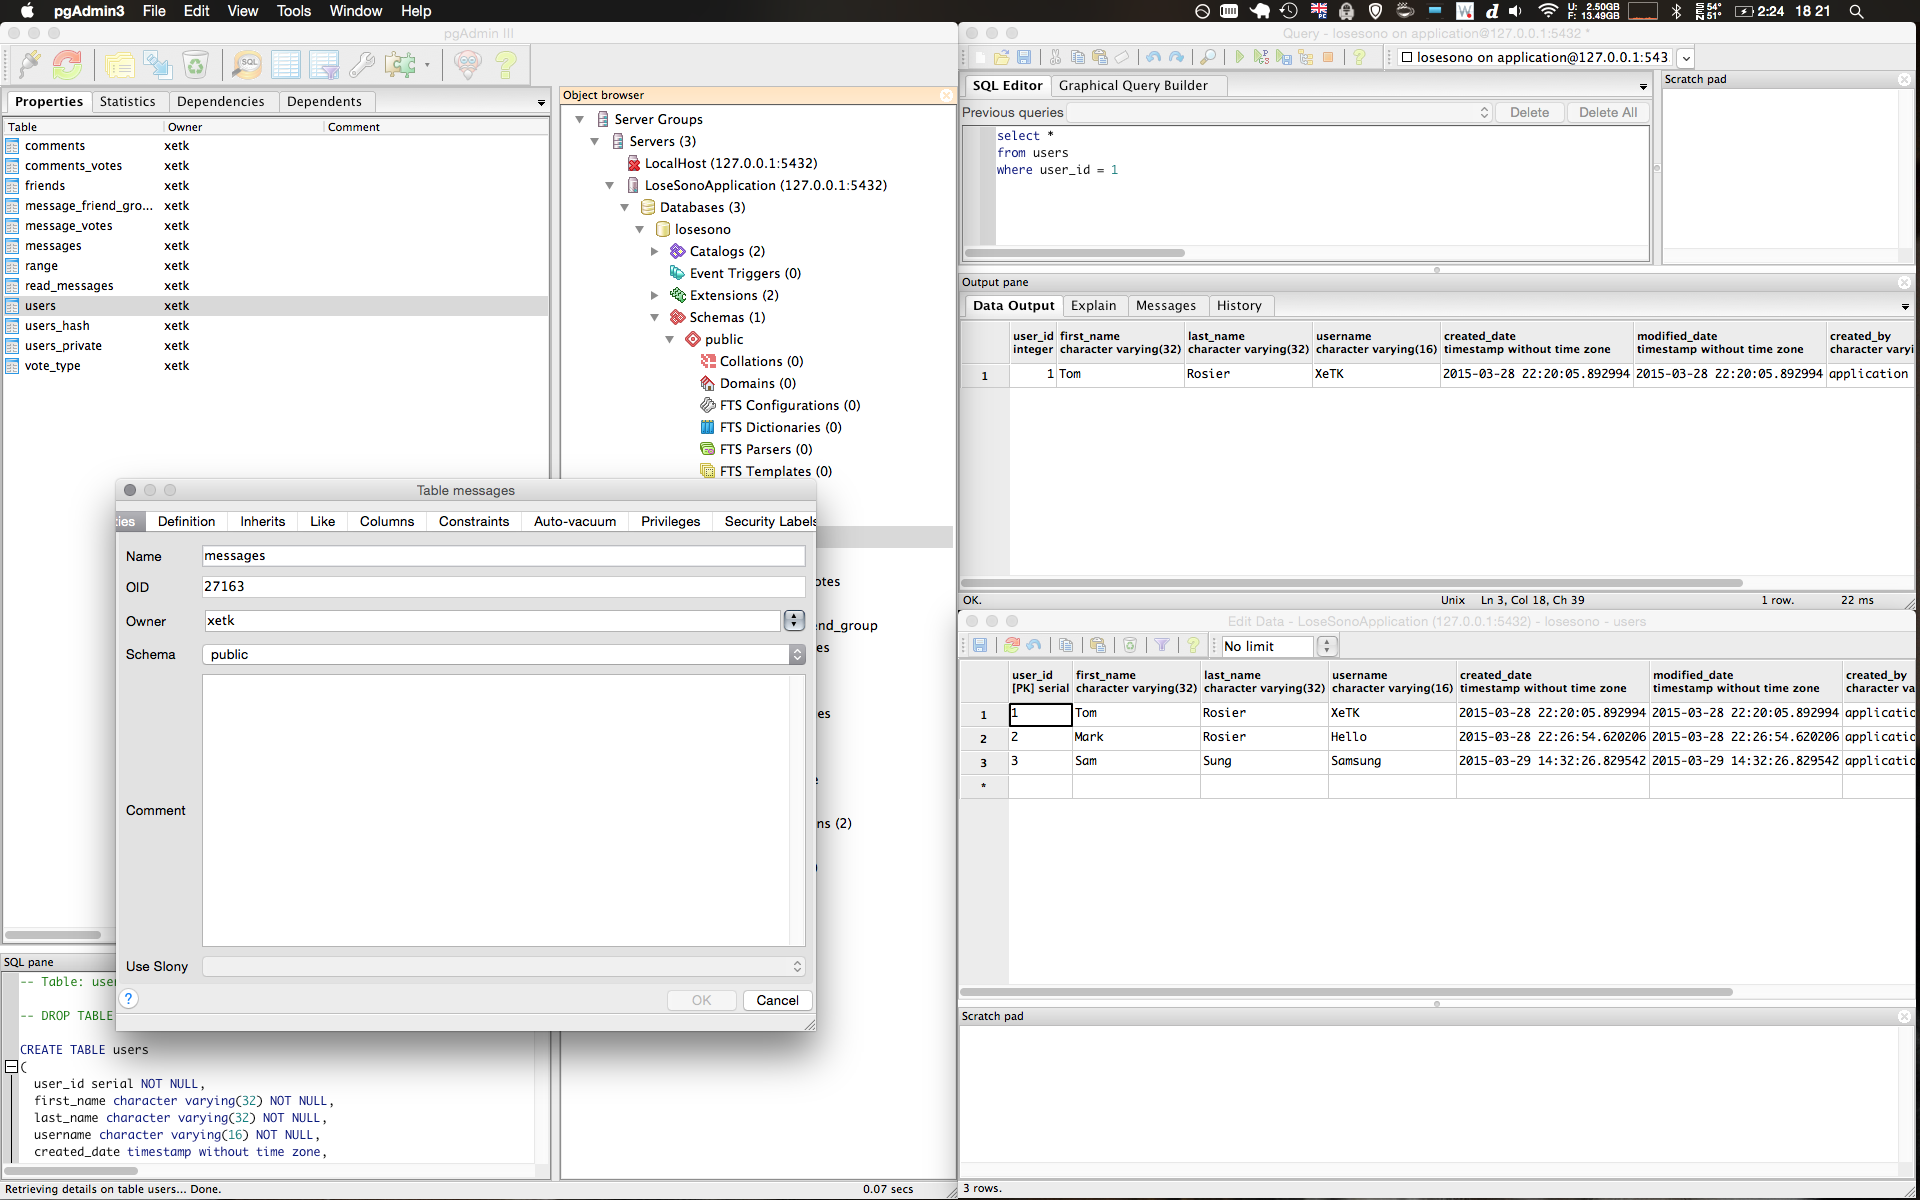
\includegraphics[width=\textwidth]{tools/pgadmin}
    \caption{PGAdmin 1.20.0}
    \label{fig:pg_admin_image}
\end{figure} 
\noindent

\subsection*{Postman}

\begin{figure}[h]
    \centering
    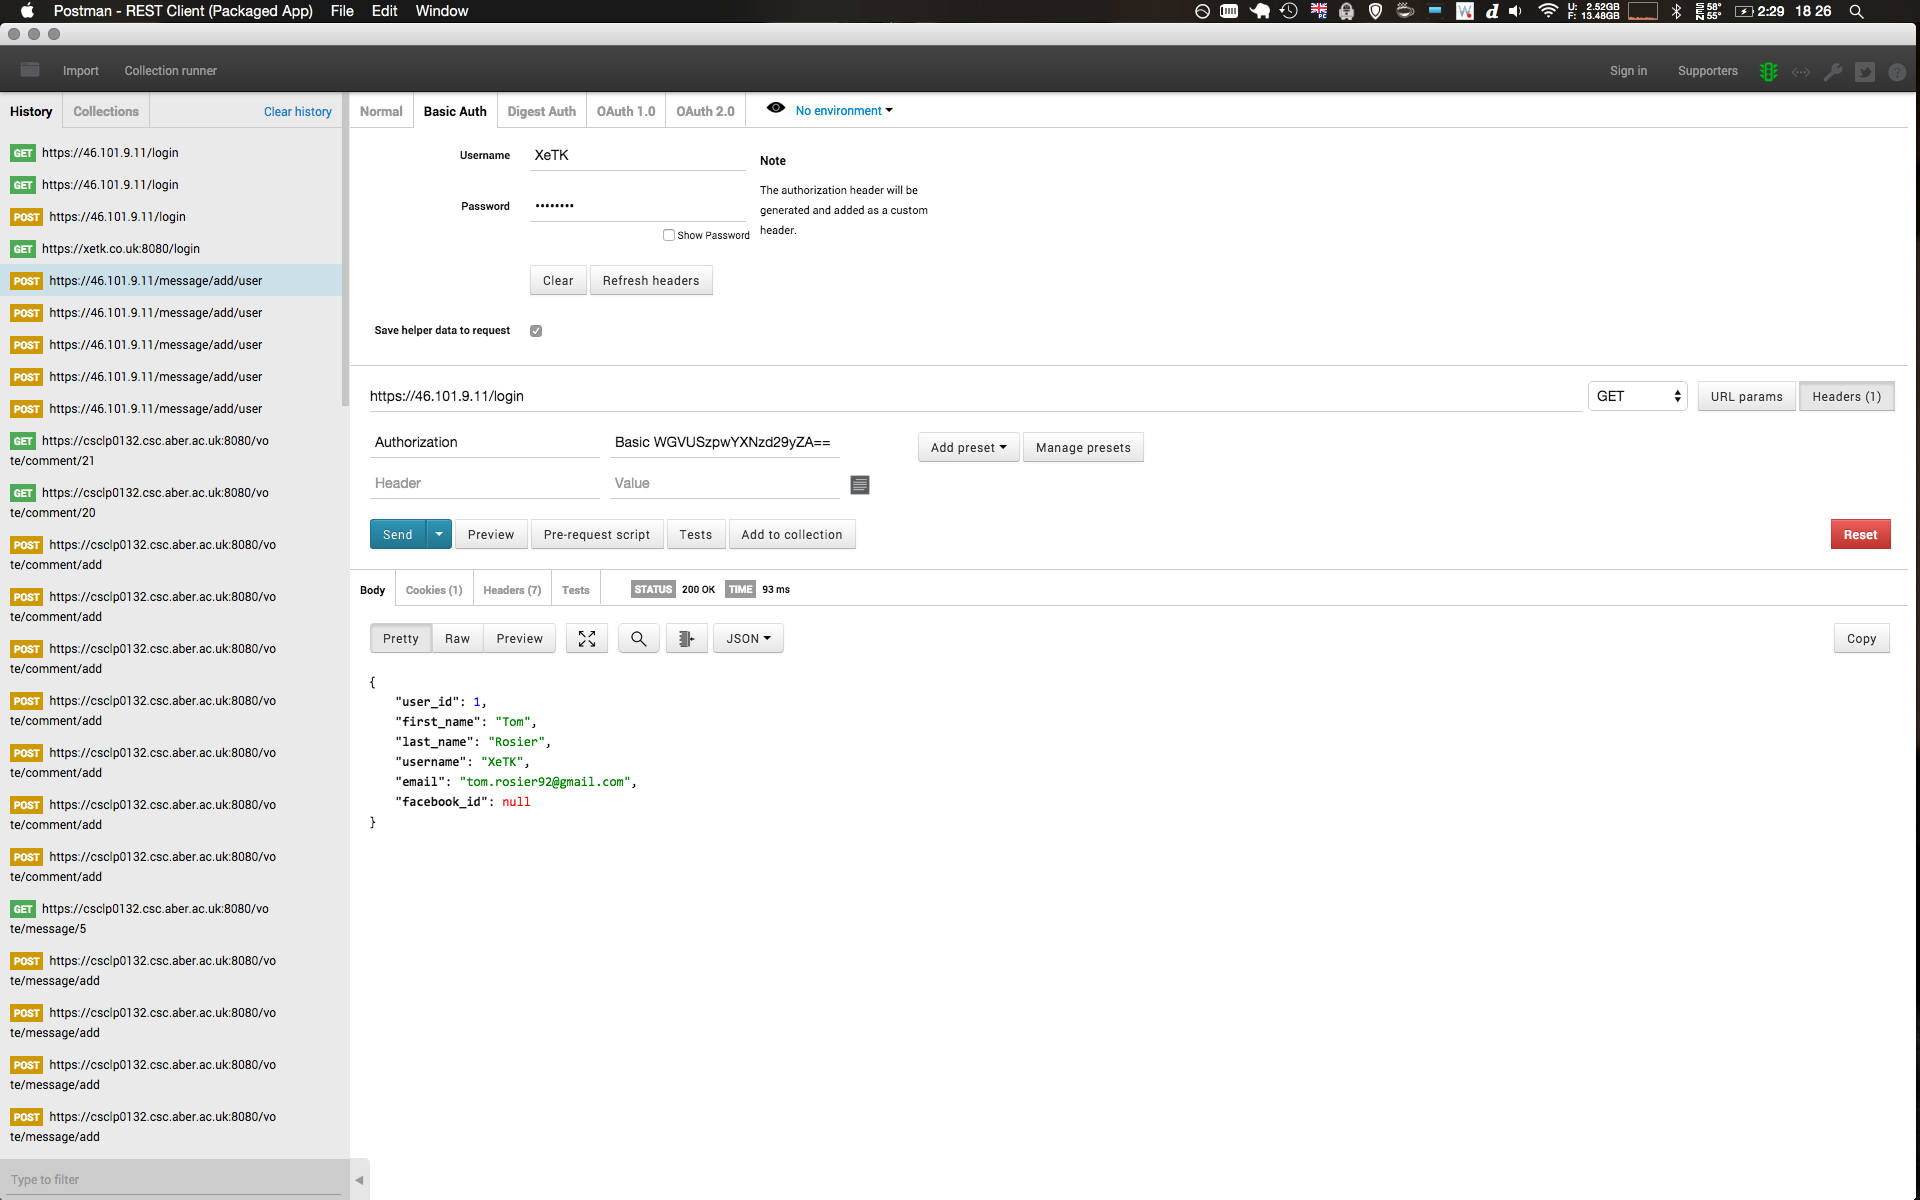
\includegraphics[width=\textwidth]{tools/postman}
    \caption{Postman 2.0.19}
    \label{fig:postman_image}
\end{figure} 
\noindent

\subsection*{Web browsers}

\begin{figure}[h]
    \centering
    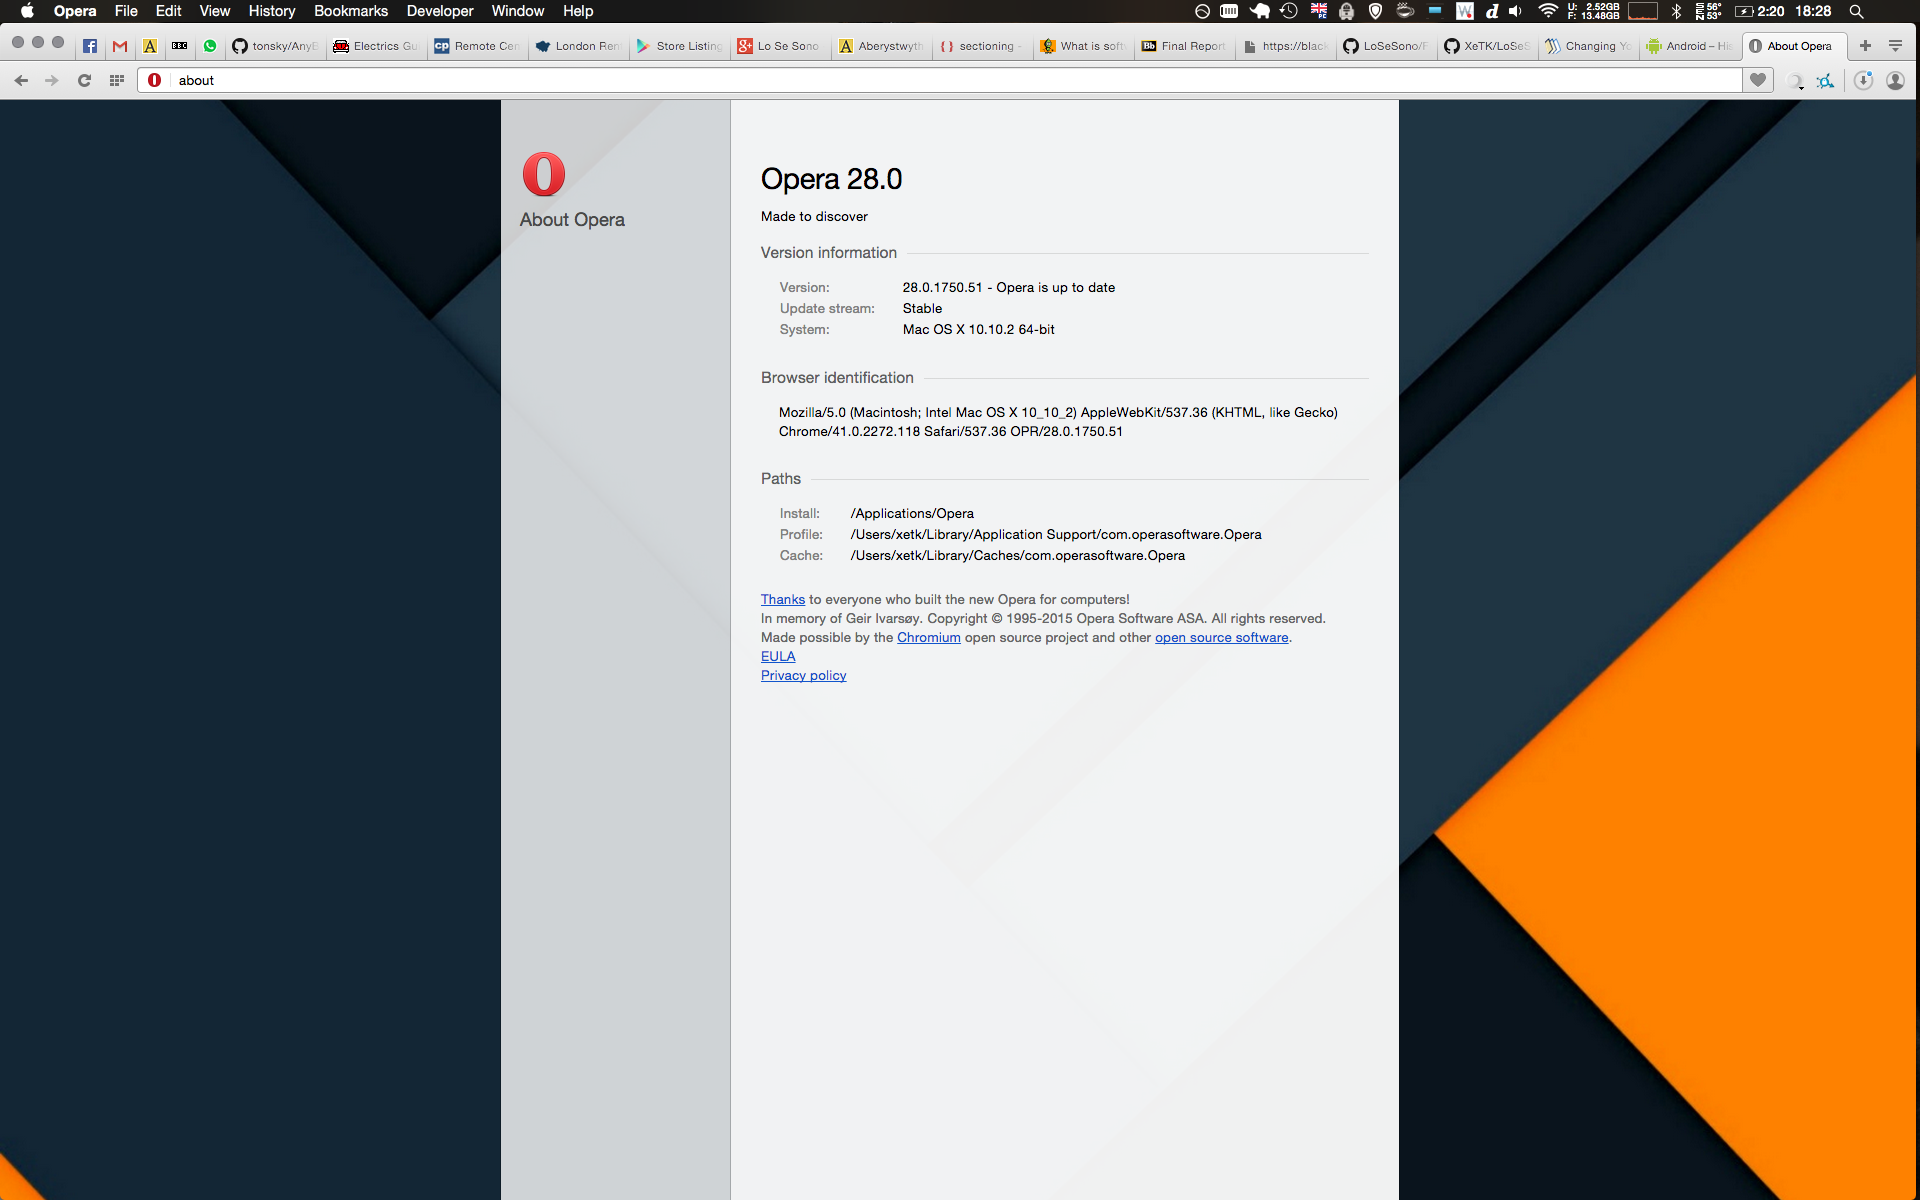
\includegraphics[width=\textwidth]{tools/opera}
    \caption{Opera 28.0}
    \label{fig:opera_image}
\end{figure} 
\noindent

\begin{figure}[h]
    \centering
    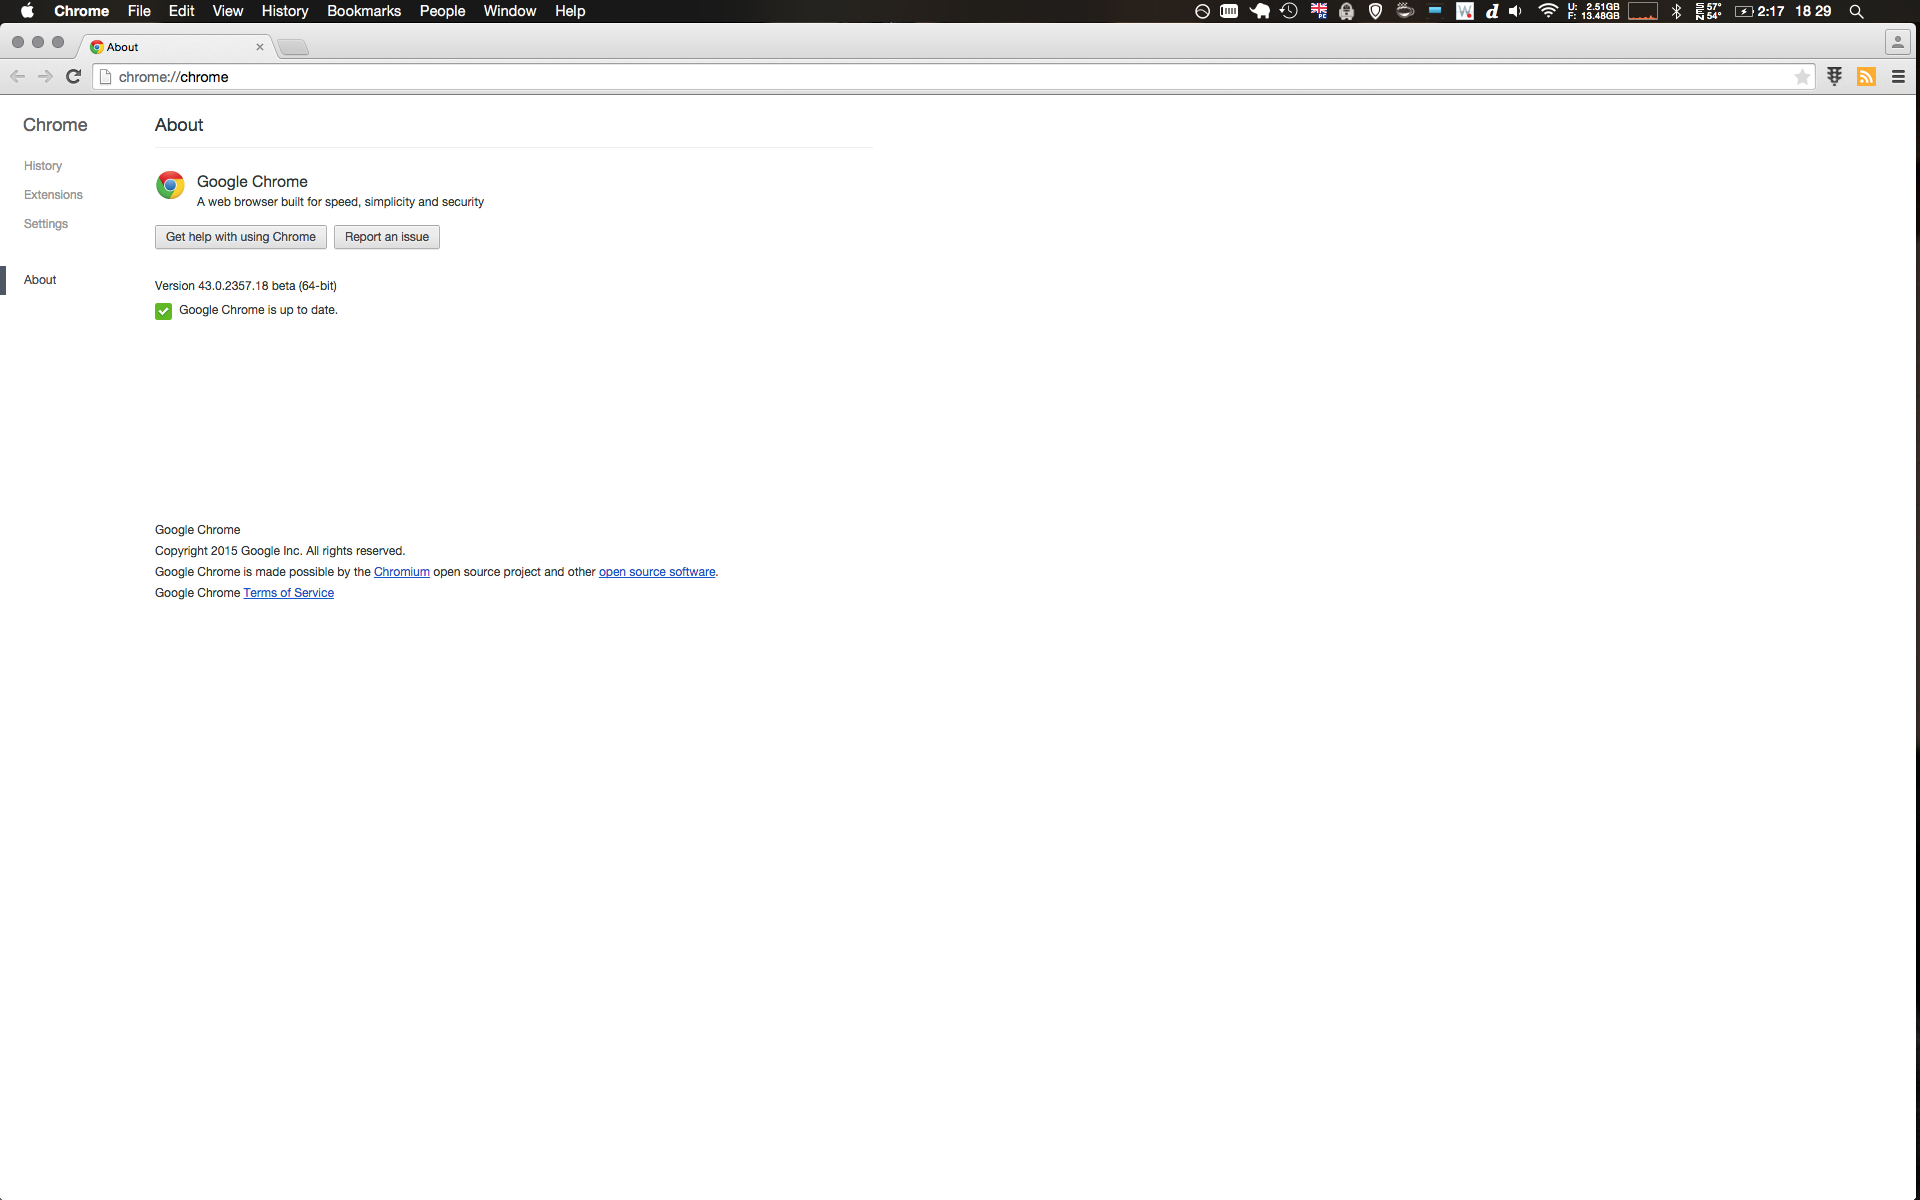
\includegraphics[width=\textwidth]{tools/chrome}
    \caption{Chrome 43.0}
    \label{fig:opera_image}
\end{figure} 
\noindent

\subsection*{Android SDK Tools}

\begin{figure}[h]
    \centering
    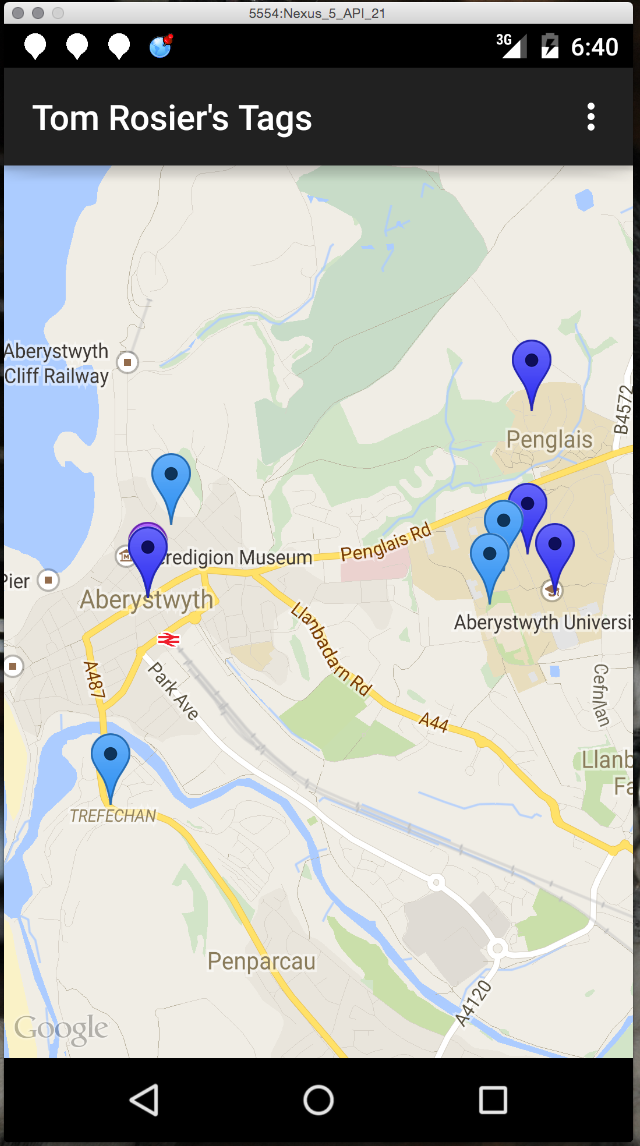
\includegraphics[width=0.5\textwidth]{tools/androidemulator}
    \caption{Android Emulator SDK 22}
    \label{fig:android_emulator}
\end{figure} 
\noindent

\begin{figure}[h]
    \centering
    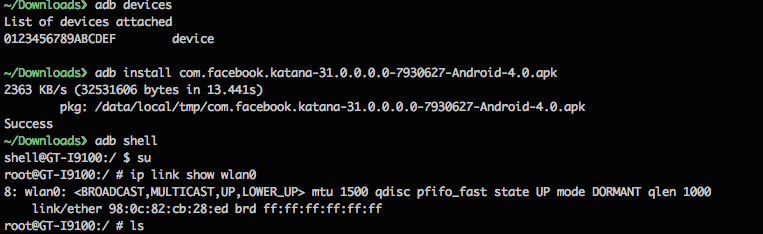
\includegraphics[width=0.75\textwidth]{tools/adb}
    \caption{Android Development Bridge}
    \label{fig:adb_image}
\end{figure} 
\noindent

\begin{figure}[h]
    \centering
    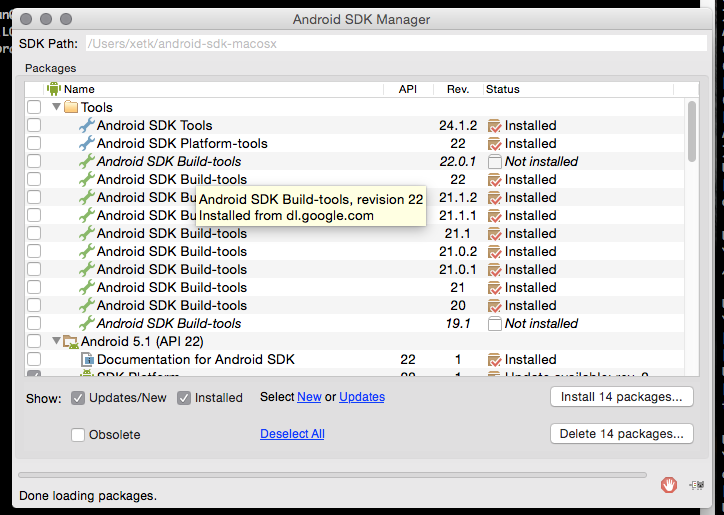
\includegraphics[width=0.75\textwidth]{tools/sdkupdator}
    \caption{Android SDK Updater}
    \label{fig:sdk_updator}
\end{figure} 
\noindent


\subsection*{PGSQL command line}

\begin{figure}[h]
    \centering
    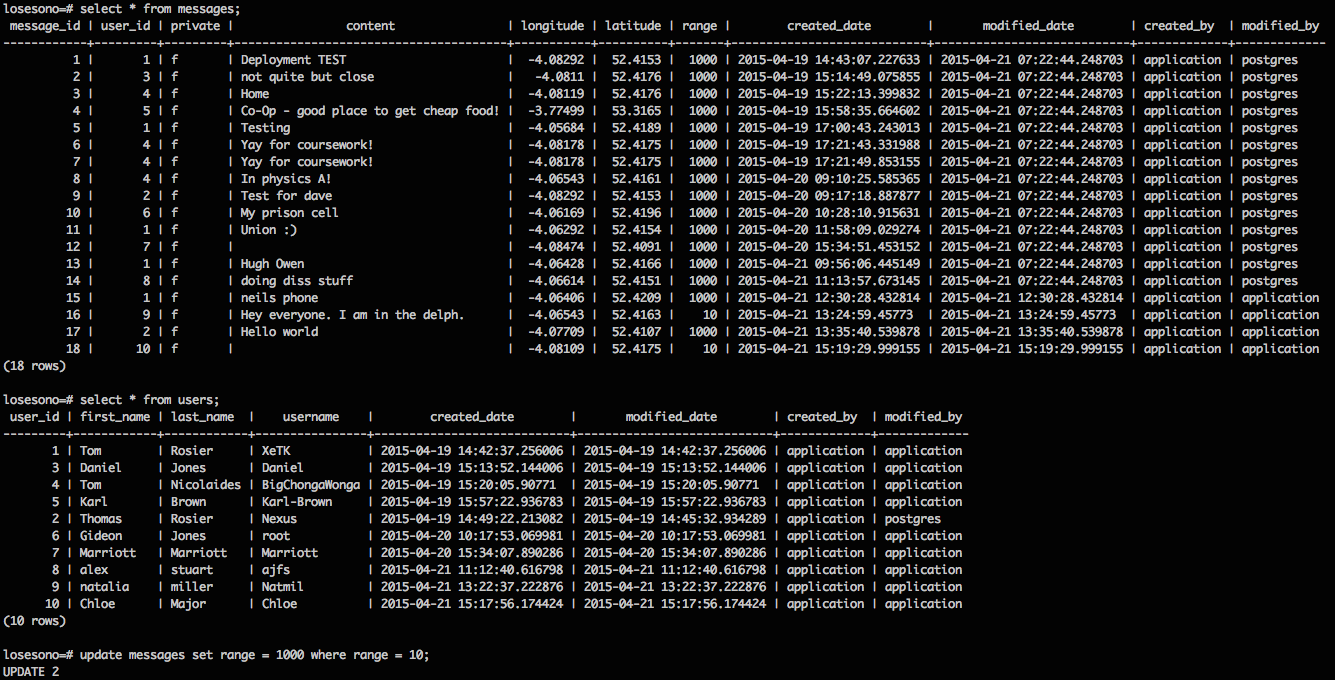
\includegraphics[width=\textwidth]{tools/pgsqlcommandline}
    \caption{PG SQL Command line 9.3.6}
    \label{fig:pg_sql_image}
\end{figure} 
\noindent


\section{Android application}

\subsection{Development Hardware}

\subsection{Environment}

\subsection{Features}


\subsubsection*{Login}

\paragraph*{Implementation}

\paragraph*{Issues}


\subsubsection*{Registration}

\paragraph*{Implementation}

\paragraph*{Issues}


\subsubsection*{Adding Friends}

\paragraph*{Implementation}

\paragraph*{Issues}


\subsubsection*{GPS Location}

\paragraph*{Implementation}

\paragraph*{Issues}


\subsubsection*{Maps}

\paragraph*{Implementation}

\paragraph*{Issues}


\subsubsection*{Posting message}

\paragraph*{Implementation}

\paragraph*{Issues}


\subsubsection*{Retrieving messages}

\paragraph*{Implementation}

\paragraph*{Issues}


\subsubsection*{Retrieving notifications}

\paragraph*{Implementation}

\paragraph*{Issues}


\subsubsection*{Comments}

\paragraph*{Implementation}

\paragraph*{Issues}


\subsubsection*{Votes}

\paragraph*{Implementation}

\paragraph*{Issues}



\section{Server side application}


\subsection{Environment}

\subsubsection{Debian based Linux}

\subsubsection{Postgres Database}

\subsubsection{Node.js environment}


\subsection{Middle tier application}

\subsubsection{Core functionality}

\subsubsection{Rest Interface}

\subsubsection{Database Connector}


\subsection{Database level}

\subsubsection{Tables}

\subsubsection{Functions}


\section{Review of implementation}
\chapter{Testing}

As with any software engineering project testing is integral to creating a well rounded and robust product that the users actually want to use. Good quality testing helps with keeping the application reliable and should ensure that the end users do not get bombarded by a vast array of issues that will ultimately hurt the application's reputation within the market place.

\section{User Testing} 

The majority of the testing for the application came from real world users or real people testing the application to find bugs or to give feedback on the designs given.

\subsection{Testing community}

For testing the application an extensive group of individuals was set up to test and stress the application to find any issues that may be contained within. The list of individuals that helped with testing the application can be found in the figure \ref{fig:test_users}. I would like to thank all of them for there input.

\begin{figure}[H]
    \centering
    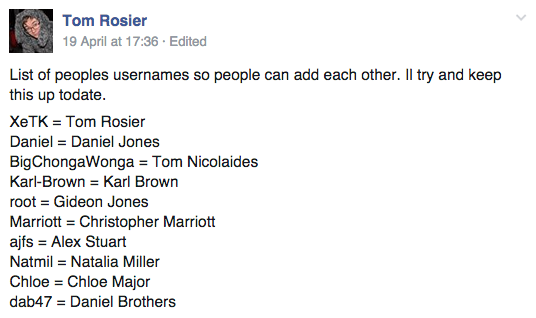
\includegraphics[width=0.75\textwidth]{testing/usernames}
    \caption{The beta test group of users}
    \label{fig:test_users}
\end{figure}

\noindent
A Facebook group was created where the test users could easily raise their concerns with the application and allow a forum for the various individuals to participate in the conversation on how to improve the design of the application and hopefully create a more rounded application for the users to use. Images of the Facebook group can be found in figure \ref{fig:facebook_group}.

\begin{figure}[H]
    \centering
    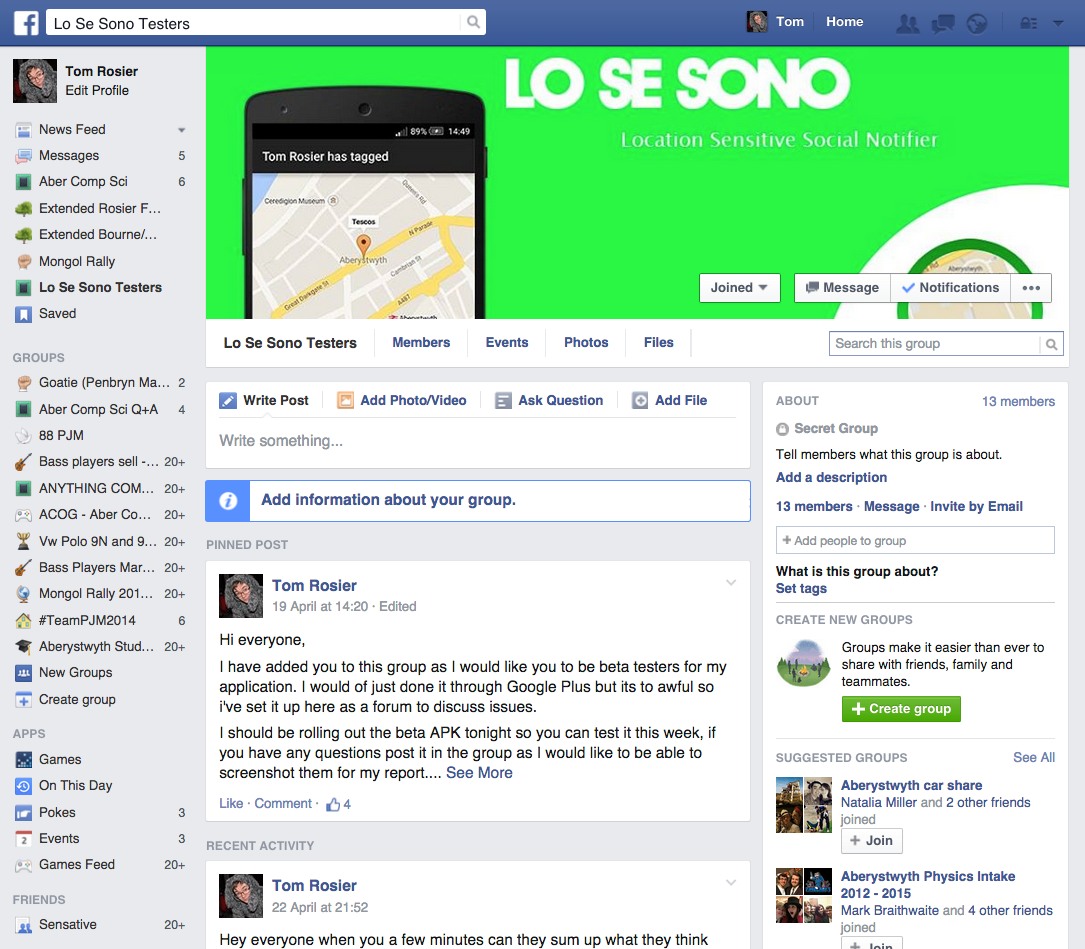
\includegraphics[width=\textwidth]{testing/forum}
    \caption{Facebook used as a forum to voice issues \& feedback}
    \label{fig:facebook_group}
\end{figure} 

\noindent
The test community was used in the very last part of the development when it was felt that the application was nearing a point where it could be used reliably by a reasonably sized group of users. It was pushed out to the group of beta testers for them to test and find issues within the application.\\
\\
It quickly became apparent that there were a number of issues contained within the application that meant that it did not behave correctly. These issues were reported through the Facebook group or GitHub where they could quickly be verified and checked for the authenticity.\\
\\
In figure \ref{fig:gideons_feedback} it shows Gideon Jones raising an issue that a person can be marked in two different places at the same time. If there is a refresh of the items on the screen it will draw the marker in two different distinct places and will lead to a confusing event for the user of the application as they will be unable to tell where the marker will be placed and one is still stuck in the older location.\\
\\
Gideon also queries if the application will log into multiple different devices, which was an aspect that was not made clear to the users of the application. The application has been designed to work on multiple devices at the same time under the same user.

\begin{figure}[H]
    \centering
    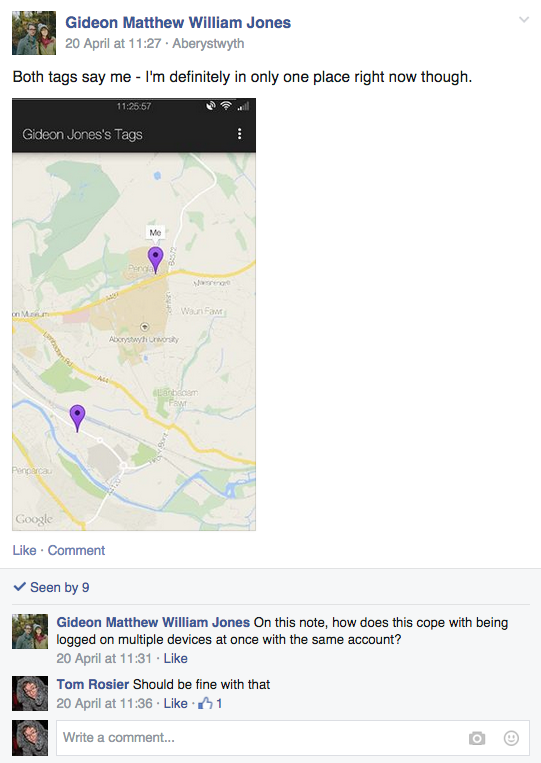
\includegraphics[width=0.75\textwidth]{testing/gideonmultiplepointers}
    \caption{Gideons feedback on issues}
    \label{fig:gideons_feedback}
\end{figure} 

\noindent
Again in figure \ref{fig:toms_feedback} Tom Nicolaides comments on the same issue as Gideon and asks for extra support from the community to verify the issue. He also mentions another issue with the application where it crashes if the GPS is not enabled when the application is initially loaded up, which has been a known issue for a large period of time, but has not impacted development so has yet to be fixed.

\begin{figure}[H]
    \centering
    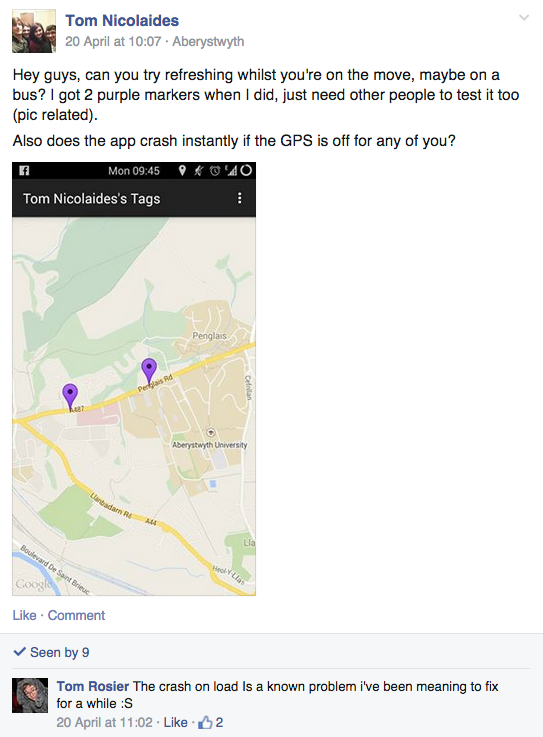
\includegraphics[width=0.75\textwidth]{testing/tommultiplepointers}
    \caption{Tom's feedback on multi location issue}
    \label{fig:toms_feedback}
\end{figure}

\noindent
The use of user based testing was a very helpful way to assess whether the application worked well in the hand of real users and to see if the concept held up as a whole and would be a useful tool for users to use in the real world. From the testing it seems that the concept works and that users do like the functionality given to the end users.

\subsection{Test Devices}

Table \ref{table:device_table} contains a list of devices used to test the application with the various points including model name, Android version, screen resolution, if they are stock or rooted (have been modified), and who owns the device. With this wide array of devices it helped test a large demographic of different devices and different versions of Android. Unfortunately, within the group of users most people tend to have a group of popular devices (mostly Samsung Galaxy devices or HTC One's) where they were very popular devices when they were released and when that group of users purchased their devices they were the best devices to buy.\\
\\
The majority of the devices were running a version of Android Lollipop and had a screen resolution greater than 720p, which made this a good selection of newer devices to work with and they should have a fairly up to date API level that the application can work with. The older Samsung Galaxy S2's and Galaxy Fame were running fairly old software by today's standard and showed some issues due to the lack of some of the newer API's.

\begin{center}
\begin{table}
\begin{tabular}{ l c c c r }
\hline
Device & Android Version & Screen Resolution & Rooted & Owner \\
\hline
Motorola G Gen 1 & 5.0.2 & 1280 x 720 & no & Mark Rosier \\
Motorola G Gen 2 & 5.0.2 & 1280 x 720 & no & Daniel Brothers \\ 
\hline
LG G-Pad 8.3 & 5.0.2 & 1920 x 1200 & yes & Gideon Jones \\
LG Nexus 4 & 5.1 & 1280 x 768 & no & Alex Stuart \\
LG G3 & 5.0 & 2560 x 1440 & no & Joe Roberts \\
\hline
Sony Xperia Z1 Compact & 4.4.2 & 1280 x 720 & no & Chris Marriott \\ 
Sony Xperia Z3 & 5.0.2 & 1920 x 1080 & no & Alex Stuart \\
\hline
Samsung Galaxy S2 & 5.1 & 800x480 & yes & Tom Rosier \\
Samsung Galaxy S2 & 4.1.2 & 800x480 & no & Tom Rosier \\
Samsung Galaxy S2 & 4.1.2 & 800x480 & no & Sam Jackson \\
Samsung Galaxy S3 & 4.4.4 & 1280 x 720 & yes & Tom Nicolaides \\
Samsung Galaxy S3 & 4.3 & 1280 x 720 & no & Daniel Jones \\
Samsung Galaxy S3 & 4.3 & 1280 x 720 & no & Chris Savill \\
Samsung Galaxy Fame & 4.1.2 & 480 x 320 & no & Neil Taylor \\
\hline
HTC One M7 & 4.4.3 & 1920 x 1080 & yes & Gideon Jones \\
HTC One M7 & 4.4.4 & 1920 x 1080 & yes & Karl Brown \\
HTC One M7 & 5.0.2 & 1920 x 1080 & yes & Tom Rosier \\
HTC One M7 & 5.0.2 & 1920 x 1080 & no & Natalia Miller \\
HTC One M8 & 5.0.2 & 1920 x 1080 & no & Chloe Major \\
HTC One M9 & 5.0.2 & 1920 x 1080 & no & Karl Brown \\
\hline
\end{tabular}
\caption{Table of devices used for testing}
\label{table:device_table}
\end{table}
\end{center}

\section{Unit Testing}

Unit testing was used within specific areas of the application, most specifically the backend API, to verify that in fact the RESTful requests are working correctly and are returning the information they should be.\\
\\
Due to the nature of Android it was fairly difficult to unit test the application as everything was very asynchronous and difficult to integrate tests into effectively. With more time and patience it is completely possible to have added in unit tests to the application, but due to early delays and issues the unit testing of these areas got left behind and would definitely need to be added to ensure that the application is working correctly.\\
\\
The Unit tests used to ensure the back end is working correctly focused on the RESTful routes of the application and verified that the changes were made to the application where appropriate or the data being returned was definitely the correct data that the user should be receiving.\\
\\
A list of the tests deployed via unit tests can be found in Appendix \ref{ch:apx_testing} section \ref{sec:test_tables}.

\section{UI Testing}

The other large area of testing carried out was seeing how the UI that had been designed and developed scales to different devices, as the device was primarily developed on a 1080p device. Due to the application only being developed to a proof of concept stage, some of the UI has not been finished to its full potential, so on smaller resolution screens, although some consideration has been made to ensure that the UI elements should fit, as you can see in figures \ref{fig:ui_scaling_home_image}, \ref{fig:ui_scaling_post_image}, \ref{fig:ui_scaling_view_image} and \ref{fig:ui_scaling_friends_image} the UI does not scale correctly with sub 1080p devices. This causes some issues with the usability of the application on these lower resolution devices.\\
\\
These issues would be fixed on newer iterations of the application as there would be more opportunity to design the UI to work on the different resolutions, with special layouts being created to add support for the lower resolution devices. This is covered more in depth in chapter \ref{ch:design} section \ref{sec:development_future_dev}.\\
\\
The UI scaling pictured in figure \ref{fig:ui_scaling_home_image} shows a best case scenario where everything has scaled correctly and the user can see exactly what is going on. The only slight difference is that the user can't quite see as much of the map on the lower resolution devices compared to the other devices.\\
\\
There was feedback from the testing stages that says the home page of the application is fairly hard to understand when coming in new to the application and that some features that should be easily accessible within the UI are not and it should be changed to make it easier to the users to find these functions. This will be changed within further development to help improve the usability of the application overall.

\begin{figure}[H]
    \centering
    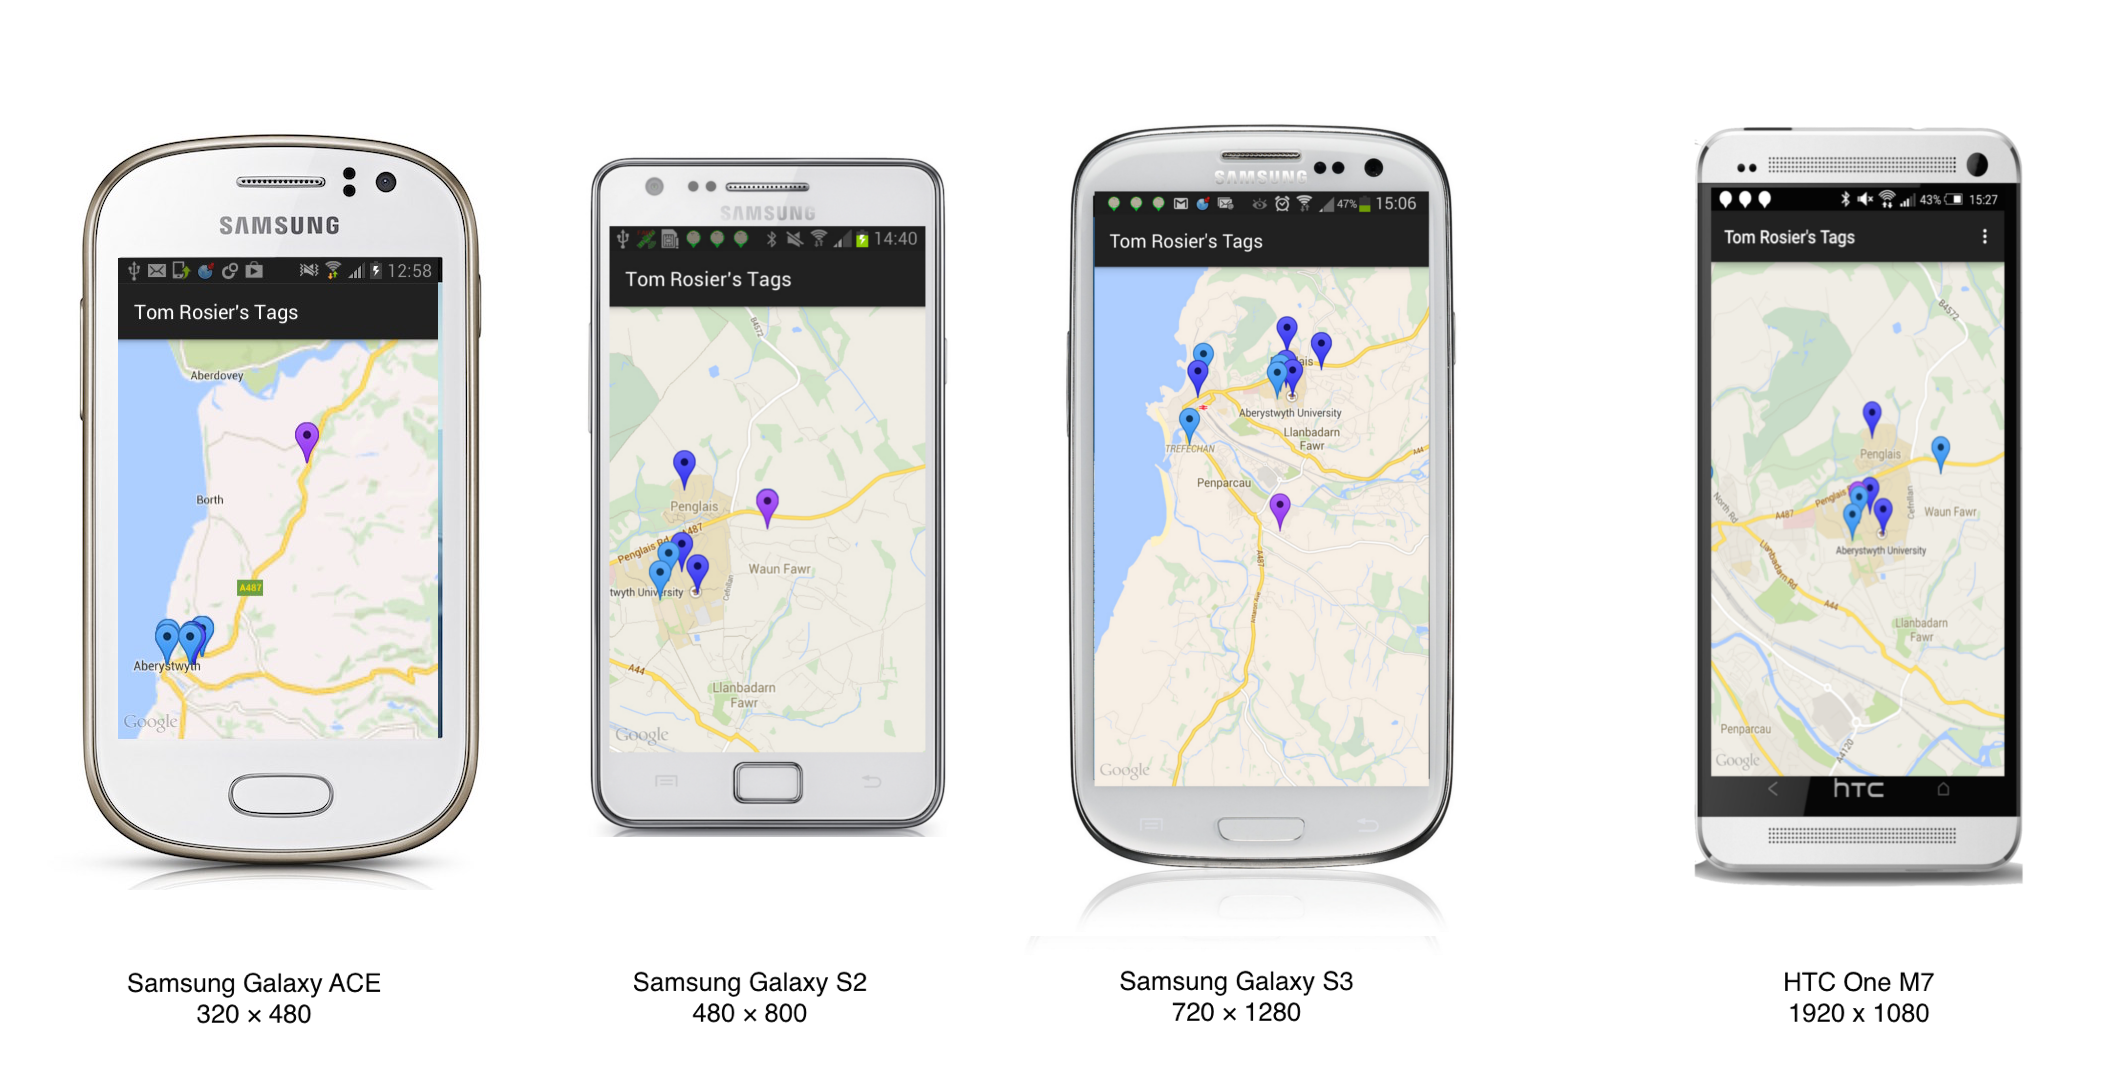
\includegraphics[width=\textwidth]{uiscaling/home}
    \caption{Home activity on different devices}
    \label{fig:ui_scaling_home_image}
\end{figure}

\noindent
The posting messages screen is one of the screens that does not scale as well on a lower resolution device compared to the other pages. It has the issue that the UI elements start to overlap and the lower screen resolution is causing issues in being able to access all of the buttons in the correct places. As you can see in figure \ref{fig:ui_scaling_post_image}, by the time we get to the Galaxy Fame the text field is overlapping the post button which causes an issue, but at least the screen is still functional and the user can still carry out the action that they were intending to do.\\
\\
The posting UI still needs some work to ensure that it can be easily understood by all the users. The UI elements at the current point remain unclear to the user and they tend to need to have to experiment to fully understand what is happening in the UI. This is down to time constraints and with more time the UI will mature to a point where it is much more usable and easy to interpret by the users.

\begin{figure}[H]
    \centering
    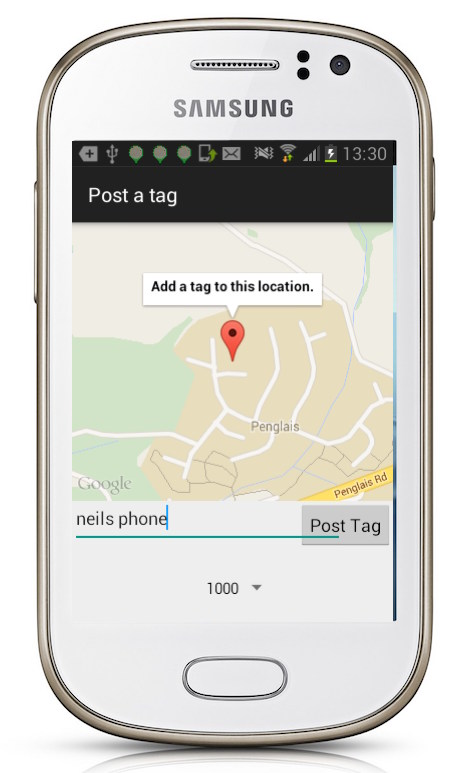
\includegraphics[width=\textwidth]{uiscaling/post}
    \caption{Post message activity on different devices}
    \label{fig:ui_scaling_post_image}
\end{figure} 

\noindent
Viewing of messages is the most complicated screen within the application and surprisingly scales fairly well on most devices, bar the Samsung Galaxy Fame, which came as a shock as there are a lot of UI elements all working together in a fairly confined space. For the smaller screen resolution a new layout would need to be designed to allow everything to be displayed correctly and in a way that is friendly for lower resolution devices. These changes could be made fairly easily and would quickly bring the application to a point where it could be used on all sorts of devices.\\
\\
These problems are caused by the restricted development time of the project and with more time these issues will be resolved. But with the short time given the application stands up fairly well with minimal testing on lower resolution devices.\\
\\
The viewing of messages UI also needs some work to help with its usability. At the current time it looks too cluttered and to be fairly confusing for the user.

\begin{figure}[H]
    \centering
    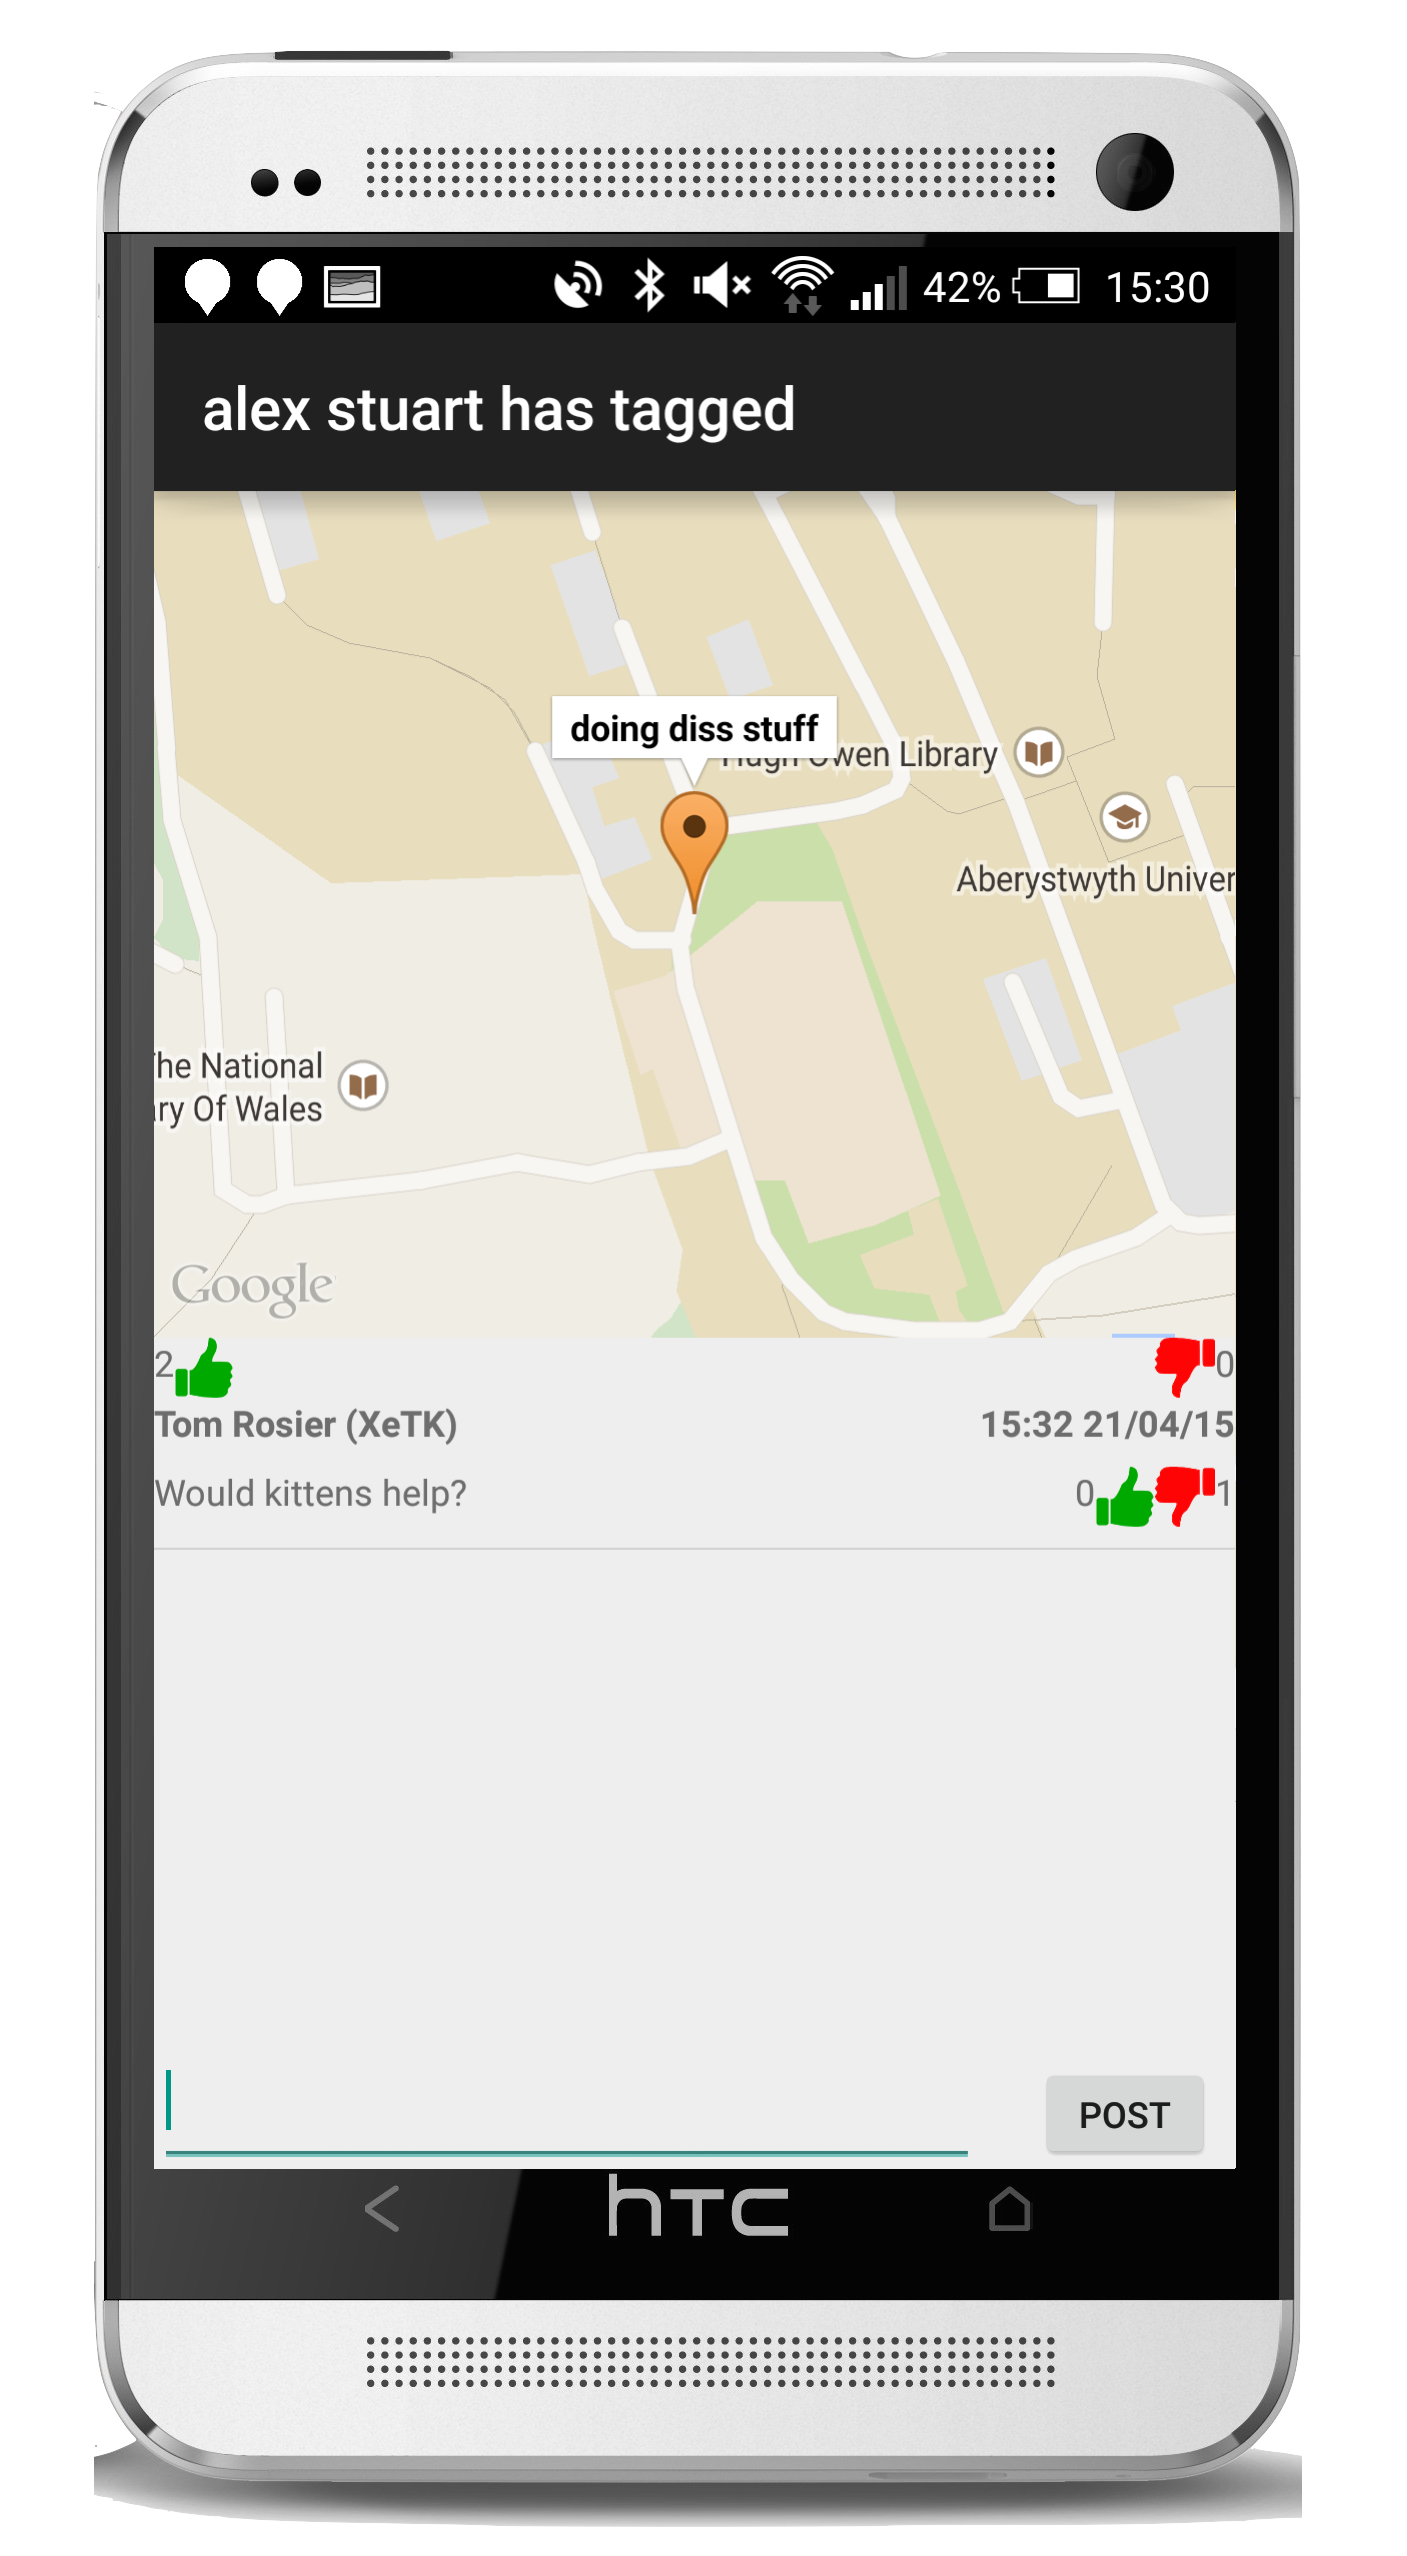
\includegraphics[width=\textwidth]{uiscaling/view}
    \caption{Viewing message on activity on different devices}
    \label{fig:ui_scaling_view_image}
\end{figure} 

\noindent
Due to the screen that adds users to a message being fairly simple, it was possible for it to scale all of the screen sizes easily. It uses a native Android element for the list design, thus there is not much that has been customised for this design, meaning that it should scale fairly effectively to the different UI's.

\begin{figure}[H]
    \centering
    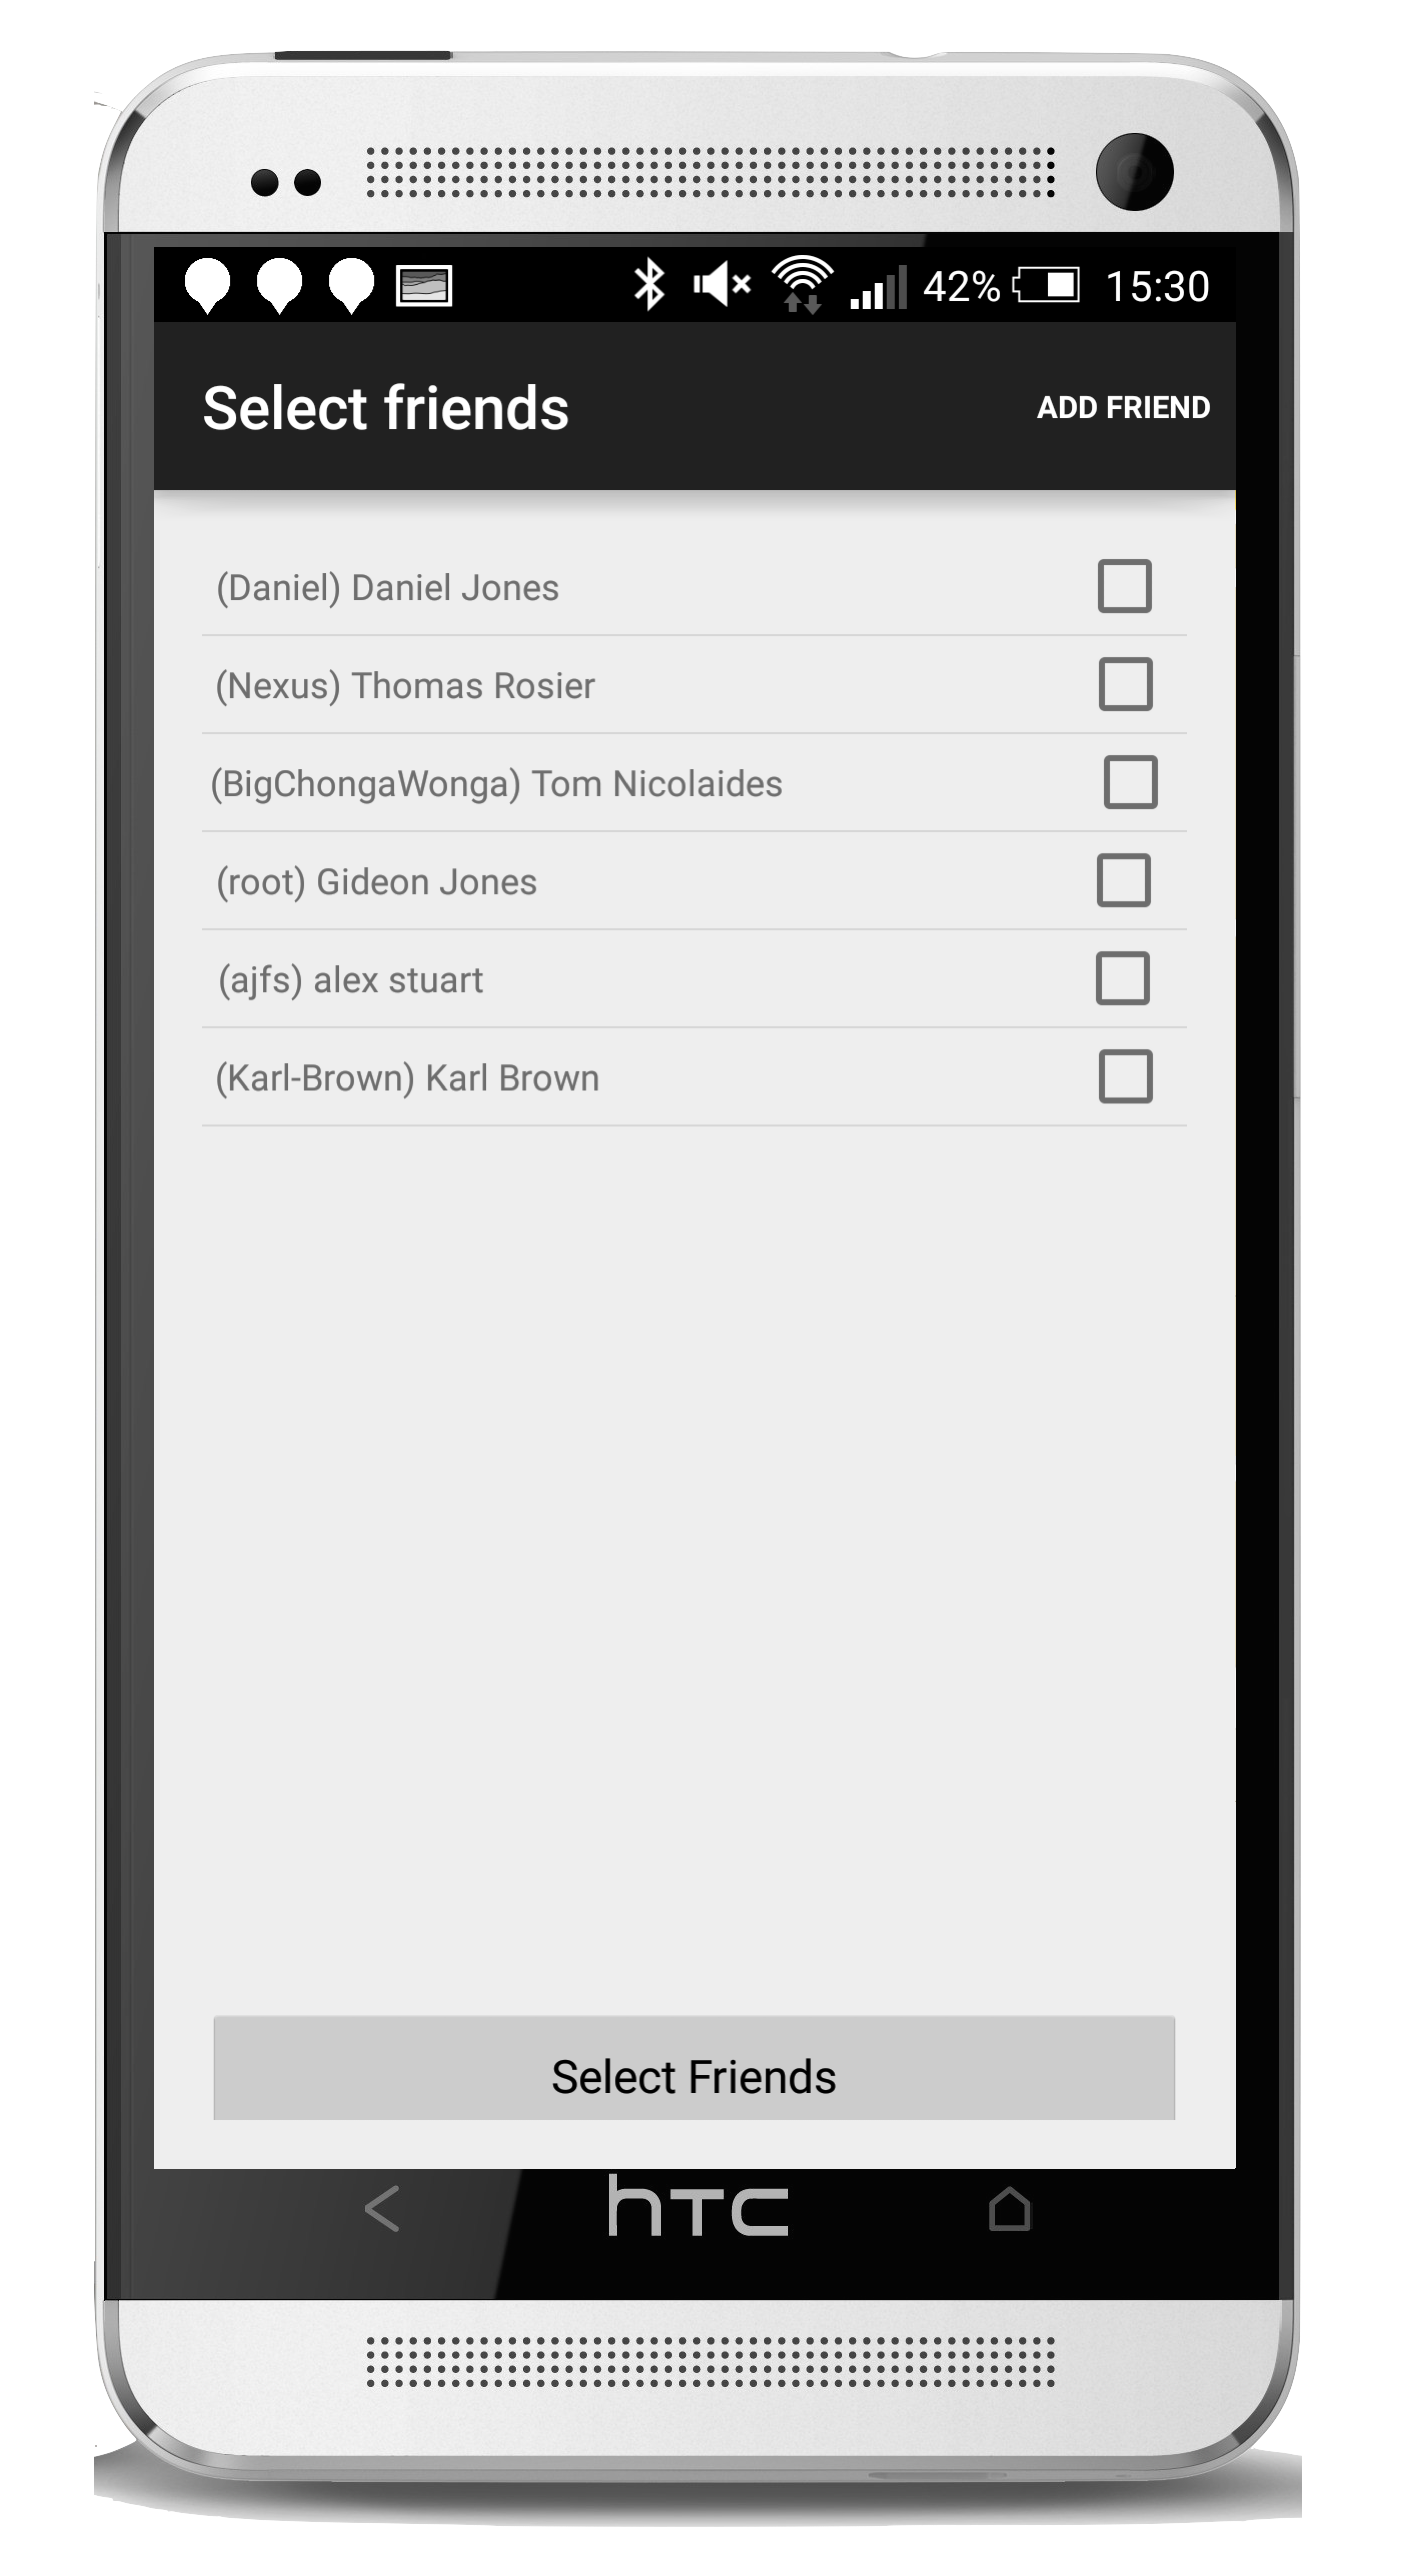
\includegraphics[width=\textwidth]{uiscaling/friends}
    \caption{Setting visibility to friends on different devices}
    \label{fig:ui_scaling_friends_image}
\end{figure} 

\noindent
The UI as it stands currently is usable but it will need more work to get it to a production standard that is expected of an application of this caliber It will require further development to get it to a point where users will want to use the application and some of the oddities of the application will be eradicated.

\section{Functionality Testing}

For each part of the application there is a degree of functionality testing needed to ensure that the application behaves in the correct manor. Each part of the functionally was tested as it was implemented to ensure it would fit in with the requirements needed to make the application work as intended within the functional requirements that were detailed in chapter \ref{ch:design} section \ref{sec:functionality}. This testing was done by the developer of the application as it was developed and development would not move on till it was guaranteed that the application worked in the way expected by the developer to fulfill the functional requirements given for a specific section of the application that is being tested.\\
\\
When the feature was deemed to have completed the testing procedure, development would shift to the next feature in the list of items to develop. The use of user testing along with the testing done by the developer would be enough to deem if the application's functional aspect had reached a level of maturity that suited the feature and if it would work correctly in a production environment. The use of unit testing on the backend application should ensure the robustness of the backend when modifications have occurred to the application to add new functionality into the application. This should mean that the functionality in the backend does not get broken when changes are made.

\section{Stress Testing}

Limited stress testing has been carried out on the application at this point in time. At most there has been 15 users using the application at any given time, which is unlikely to have put a major strain on the system. So far, although there has been issues with the backend application, this seems to originate in the Sequelize library, but more work needs to be undertaken to diagnose where exactly the issue is coming from. For now, allocating more ram to the VPS solves the issue, but it would be preferred to try and fix the issue fully. But again this is a point to cover in future development and not at the current version that the application is in.\\
\\
The user testing has been used to stress out the application screens and ensure that they are robust and will take abuse from the users. Some of the users that are testing the application are fairly technical and have tried various SQL attacks and Overflows to try and break the application. This may be a place where automated testing could be added to test the various parts of the user experience to see if they fall over from various types of attacks, including buffer overflows and SQL injection attacks.\\
\\
Building up the testing suite for the application to ensure that all parts of the application are protected from various malicious attacks and large amounts of data requests, should ensure the application is robust within a production environment. Additionally, it will ensure that the user's experience will be good and they should not be disappointed with the experience provided by the application as a whole.\\
\\
The use of stress testing should ensure the application will have capable error handling, along with being robust, which will ultimately lead to the application being readily available and up for all to use at any time that they want to use it. Work needs to be continued to get the application to this stage, but due to being a proof of concept application the robustness in the application is lacking and more work will be needed to turn the project into a robust product that users want to use.
\chapter{Evaluation}

This chapter will give critical evaluation of the project as a whole along with giving feedback on the various elements that made up the project.

\section{Application}

Firstly, critical evaluation will take place of the application that was developed as part of the project, illustrating the good points and the bad points of the application, explaining what was done well within the application and what could do with improvement to make the application better as a whole.

\subsection{Achievements - Good Bits}

This section will talk about parts of the application that were thought to have been executed well or were positive parts of the project. It will also discus the parts of the project that the developer was specifically proud of.

\subsubsection{User Feedback}

The overall feedback that was received from the users was very good and gave a good indication that the application was on the right route to becoming an application that users want to use for the various location based messages. Thomas Nicolaides wrote "I think the application is a great concept, and it fills a niche that nothing I've found previously has. I definitely would use it when it becomes available to more people." This gives a good idea that the concept is something that users want to use. Daniel Jones wrote "{STICK QUOTE IN}" .\\
\\
This feedback is a great accomplishment and it is good to see the user community is interested in the application as a whole and that it could potentially grow into an application that a lot of people want to use. A large part of the general feedback received from showing the application has been fairly positive and people seemed to be very intrigued by the idea and want to see a fully fledged application to try out.

\subsubsection{Database Design}

The developer of the application is very happy with the way the database has been designed and the design created at the very start of the project seems to have exceeded its expectations, with very minimal modifications being made to it to make it suit application design. The design has matured and grown into the fully fledged application that we see detailed in this document.\\
\\
The design is very robust and copes well with the growth of the application and it should be very easy to add on new functionality to the database as the application grows and matures to become a production ready application. Its simplicity and low coupling should help with other developers' understanding how everything links together.\\
\\
Database functions also help to complete the database part of the application, helping to keep database type tasks segregated from the middle tier application. This should in turn help with security and performance which are key points to the application that want to be kept as robust as possible to help with the stress of users using the application.

\subsubsection{Choice Of Technologies}

For the most part the choice of technology was right. The use of PostgreSQL and HAPI.js/Node.js suited the backend development down to the ground, making development fast, along with providing the features that were needed to get the job done quickly and effectively.\\
\\
PostgreSQL lived completely up to the developer's expectations and gave many more useful features than expected. Its robustness can not be faulted for this project, along with the advanced features offered that included integrated JSON parser, advanced database functions along with built in security features with advanced hashing and encryption algorithms which made making the data secure a breeze.\\
\\
HAPI.js and Node.js together made the perfect backend for the application, being extremely flexible and versatile, with a great developer community behind them which were rearing to help anyone using their API's. These frameworks worked perfectly and did everything that was asked of them in well structured and well documented ways, which ultimately helped speed up the development of the application and create a better product at the end of it. The stability of the Node.js platform has been excellent as well, with very minor issues that stopped the application behaving as intended.

\subsubsection{Dynamic Loading}

Dynamic loading of routes within the backend application was a great time saver and a really interesting concept to get working. The developer may not have developed it exclusively for this project, but it was suited perfectly for loading in the routes for the RESTful services, which meant that no modifications were needed to be made to the supporting code to make it load in the new routes into the application which add the additional functionality needed to carry out the advanced features within the GUI.\\
\\
The use of a Dynamic Route Loader should help make the application more flexible to change in future and allow people to add on new functionality with ease, without having to modify the underlying code. This should also mean that it will be very difficult for new bits of code to add in bugs to the underlying infrastructure.

\subsubsection{Viewing \& Posting Tags}
\label{sec:viewing_posting}

One of the best bits of the application is the ability to quickly and easily post new messages within the application with a very clear and simple UI that shows exactly where the post will be placed on the map, with a simplistic text entry system that allows simple and very straightforward ways to add in a new message to the map.\\
\\
The UI for viewing messages is as simple as it can be and shows all the relevant information needed to portray the information assigned to the location on the map, with the ability to leave comments and vote on the specific point being very interesting or not. This is a great way to get the users to interact with the various points that have been left on the map, which will be important to get users to interact with the application and ultimately build the customer base.\\
\\
The map shows exactly where the tag has been left on the map and is a very good visual cue on the viewing messages screen to illustrate where the tag is and what it means to the user. This helps break up the screen and helps to keep the idea interesting, even if the user is not interested in the social and commenting side of the application.

\subsubsection{Comments \& Voting}

Commenting and voting as mentioned in the section \ref{sec:viewing_posting} are very integral to the user's participation within the application and are some of the features that the developer is most proud of, as they give a framework for users to collaborate and to leave insightful comments on the posts that have been left on the map.\\
\\
Getting the user experience right for comments was a fairly complicated procedure as there are a lot of UI elements that make up the comment sections within the application and getting them all to align and work together is a fairly difficult procedure as there also many different screen resolutions to tailor the application to work with.

\subsubsection{Notifications}

The notification section of the application is a fairly well thought out and interesting part of the application. It uses some interesting algorithms to ensure it notifies the users at the correct points in time. It does need some more work to make it a fully rounded part of the application, but it is clear to see the potential of the notifications within the application. They give clear alerts that tell the user exactly what is needed to be known to tell them about nearby tags.\\
\\
Notifications do need some work to make them better at saving power and clearing at the appropriate times, but it is clear to see how they engage the users to interact with the application and actually get a response out of the user. With a bit more work it will be an integral part of the application that users will appreciate.

\subsubsection{Project Concept}

The greatest success of the project has to definitely be down to the concept behind the application. It seemed to not have been done prior to implementing this project and the proof of concept application created from this project seems to prove the idea works and that people want to use the application.\\
\\
With some further development it is clear that the concept can be turned into a product that people will want to use and could quite potentially become a fairly popular application out in the market place, which would be a crowning achievement of the project and would make the developer immensely proud.\\
\\
The concept has come a long way since the early development of the project and it will be interesting to see how the application matures with time.

\subsection{Limitations \& Potential improvements - Bad bits}

In this section the limitations of the application and what could be improved will be discussed, it will detail what parts of the application were not up to the standard of the developer.

\subsubsection{Testing}

Testing is one part of the project that the developer does think that needs some improvement, more focus should have been given to it in the early part of the project to ensure that the application had good test coverage.\\
\\
Automated testing would help with ensuring the robustness of the application and check if any regression had happened within the development of the application which would result in a less robust application. With more time the use of automated UI testing could of aided to see if the UI worked correctly on different devices, along with unit tests to ensure that the code base remains robust and stable.\\
\\
The testing issues can be partly blamed on the limited time given for the project and the constraints this placed on developing the application it was felt although maybe this shouldnt of been the case to focus on just developing a working application to prove the concept that trying to make the application more robust from the start with slower progress overall but leading to a much more robust platform with less functionality by this stage in the project.

\subsubsection{Android}

The initial choice to use native Google Android may been a poor judgment to have made, it required re-learning a programming language and to learn a whole new framework along side that, a significant amount of time and effort was spent trying to get a grips on Android development and with hindsight it is clear that PhoneGapp may have been a much better route to go down even if it isn't as mature as the native libraries.\\
\\
Androids innate instability and development complexities that it present are a very big turn of as a developer as a lot of time is wasted in trying to get the application just to run, and what seem to be trivial elements of the design seem to take a very long time to implement for example to implement a list within the UI requires 3 classes to make it function correctly, all with modifications to make them suite the specific need.\\
\\
Phone Gapp uses the same language and framework as the backend application Node.js and uses standard web standards for example HTML, CSS \& JavaScript for its front end work. It is unclear if using Phone Gapp would of saved any pain or time in the development of the project, the developer wishes they had done more research into Phone Gapp at the beginning of the project and had done more spike work to determine what platform would be best to developer for.

\subsubsection{Confusing UI}

Some of the feedback given by the user community that tested the application has said that the User Interface can be confusing and inconsistent at other points leading to confusion which means that people struggle to understand the application and how to do tasks within it.\\
\\
The main home page seems to have caused a lot of confusion as initially its very unclear how to post a message and how to differentiate between the different users tags. This can be very disorientating for new users as they are a bit overwhelmed to start with and do not know how to interact specifically with the application.\\
\\
With more development and maybe with a developer that is better experienced at UI design or design in general looking over the application it will be easier to design and set out a design that will be less confusing for the user to use.

\subsubsection{Actively Negative}

One query that was raised by one of the users of the application that the message \& comments systems voting system seems to be overly negative and users can be actively negative towards a post rather than passively negative by choosing not to up vote a post, they are being actively negative by pressing on the down vote button.\\
\\
By using negative voting it encourages a negative environment and could show negative reenforcement which could ultimately hurt the users of the application and they may feel that they are being actively targeted and that all of there actions are bad.

\subsubsection{Error handling}

The error handling problems are in the same vain as testing as it was felt with the application should be completed to a proof of concept stage and that any extras should be left to further development, but the developer wishes they had spent more time on making the application being robust rather than rapidly developing the project to a proof of concept stage were the underlying code is not robust and will need to be gone over thoroughly before the application could be released.\\
\\
Much tighter error handling and coping strategies need to be implemented into the application before it can be released to the public as at the moment when issues happen the application is fairly likely to fall over and not give useful feedback to the user explaining what has happened for to cause the action to fail.\\
\\
With more time and further development theses issues could easily be resolved and the application should reach a maturity that means the application can be enjoyed by the general public.

\subsubsection{GPS accuracy}

As mentioned in chapter \ref{ch:background} section \ref{sec:origin} there are some issues with the accuracy of GPS, this is not really a issue but it is a noted problem with the idea as a whole as with the accuracy as it stands its not possible to do fine marking of locations, thus would be useless if the were a load of locations very close to each other that need to be marked by users differentiate between them, for example if there was a row of shops and each of them had a marker outside them telling what they are.\\
\\
It could be possible to use a Blue Tooth dongle with the application to give much more precise positioning, but this would require extra work and defeats the concept of the application working without any external hardware which was one of the main aims of the project as a whole.

\subsubsection{Mapping With Multiple Pins}

This is a issue with the Google Maps API rather than the application but there is a issue where that if there are multiple tags on the same location then its very hard to differentiate between the different tags that have been left on the same placed.\\
\\
The issue could be resolved with a bit of creative thinking from the developers end having a pin that pulls up a notification list with all the tags that are stored in the same area, this problem can be resolved in further development like most of the flaws within the application, more time is needed to polish the application.

\subsubsection{Application Completeness}

As mentioned in multiple other sections of this document the applications is far from being complete to a level where the developer is happy to release the product to the general public, the application that will be included with this report shows that the concept works and has great potential, but ultimately the application will require fair amount of work to get it to the state where it can be used by members of the public.\\
\\
Without the delays throughout the project the developer does not think that the application would be much more complete than it already is and it genuinely requires a fair amount of time to be spent to make it a viable product, the end of the dissertation does not mean the end of this project the developer has decided that they want to continue development of the application and hopefully create something that will be used a large amount of people.\\
\\
The project has had a fair bit of interest from people that are interested in helping with development and create a application and community that will work in the real world and will be a viable idea for real people.


\section{Developers performance}

This section will be assessing the developer's performance throughout the project, giving critical feedback about what was done well and what could have been done better to make the project better as a whole.

\subsection{Positive - what was done well}

This section will cover in detail what the developer thought that they did well to help with the development of the project and what they were specifically proud of.

\subsubsection{Risk Assessment}

For the project it was apparent that some risks would have to be taken to get the application to a workable level. There were stages in the early development of the application where it was felt that some of the implementation for the application was behind schedule, thus some risk assessment was needed to ensure that the project would not fall behind in the development stages.\\
\\
At the point of the midway demo it was felt that the project was falling behind and there was not enough to present. Risk assessment was used to prioritise what parts of the application needed to be completed to have a reasonable demo to show at the midway point. It was decided that the user must be able to login by this point, along with send a message to the server with the GPS coordinates of where the user was. This functionality was successfully implemented by the time the midway demo occurred, leading to a very successful demo.

\subsubsection{Priority Assessment}

With the time constraints of the project being fairly low, a plan needed to be created to ensure that the project would not be at risk of failing. It was decided that the application should be developed to a proof of concept stage which should enable user testing to occur to give an indication of whether the concept behind the application works.\\
\\
With the limited time hard decisions were made to make sure the application would reach a point where it could be tested by real users. This meant that only the most important features stayed for the development of the application. It was essential that the posting and viewing of messages were complete, along with the ability to see the list of notifications in the surrounding areas. They are not quite as robust as the developer would like but the decision was made to prioritise getting the implementation there rather than making the application completely robust to all known issues.

\subsubsection{Test Community}

Setting up a community to test the application was a novel idea for the development of the application. It got good coverage of the application and helped uncover bugs and issues that the developer would have not thought of or encountered. This also gave a much broader range of devices to test the application on and ensure that the users had their voice heard when ideas for improvements are given.\\
\\
The test community has been a fun way to get feedback on the application and to get real user's feedback on the concept, which has helped improve motivation and willingness to work on the application, as it shows people are interested in the concept and that people actually want to use the application for real world tasks.

\subsubsection{Problem Solving}

Problem solving throughout the project has been strong. With every problem there has been a solution put in place. A large proportion of the early development of the project was spent problem solving various Android devices and getting them up to a point where they could be used for development. This required large amounts of time spent learning the SDK documentation and reading a fair number of blog posts on how to fix various issues within Android and joining the points from all these resources showed strong problem solving initiative.\\
\\
The use of strong problem solving abilities were used when trying to resolve various issues throughout the development. For example, when there were some issues with the RESTful interfaces returning the wrong status, even when they were doing the correct action. The problem looked like it was originating within the UI as when mocking the interface it looked to be returning the correct information, but after digging through each layer of the application it became apparent that the problem was residing in the backend of the application, not the front end, and with a simple tweak it was possible to get the application working correctly.

\subsection{Negative - what could be improved}

Contained within this section is what the developer thought they could of possibly done better to aid with the development of the project as a whole and ultimately created a better product. 

\subsubsection{Overly Critical}

\subsubsection{Time Management}

\subsubsection{Methodologies}

\subsubsection{Motivation}


\section{Overview}


% add any additional chapters here

\setemptyheader
\addcontentsline{toc}{chapter}{Appendices}
\chapter*{Appendices}
\pagebreak

% start the appendix - sets up different numbering
\fancypagestyle{plain}{%
%\fancyhf{} % clear all header and footer fields
\fancyhead[L]{\textsl{Appendix\ \thechapter}}
\fancyhead[R]{\textsl{\leftmark}}}

\appendix
\fancyhead[L]{\textsl{Appendix\ \thechapter}}
\fancyhead[R]{\textsl{\leftmark}}
\fancyhead[C]{}
\fancyfoot[C]{\thepage}
\renewcommand{\headrulewidth}{0.4pt}
\renewcommand{\chaptermark}[1]{\markboth{#1}{}}

\fancyhead[L]{\textsl{Appendix\ \thechapter}}
\fancyhead[R]{\textsl{\leftmark}}
\fancyfoot[C]{{\thepage} of \pageref{LastPage}}

% include any appendices here
\chapter{Third-Party Code and Libraries}

This appendix will detail 3rd party code and libraries used within the application, it will explain why they were used and will accredit the author.

\lstjava

\section{Android application}

\subsection{Libraries}

\subsubsection*{Google Maps API}

This library \cite{Google:MappingAPI:2015:online} was integral for all of the maps within the application application and was very flexible in allowing modifications to be made to show details on the map. The Google Maps API is licensed under the Apache License v2.0.

\subsubsection*{Android Asynchronous Http Client}

James Smiths library \cite{JamesSmith:AjaxRestLib:2015:online} has been integral to all of the HTTP requests made from the Android application to the backend in a Asynchronous manner, this library is also licensed under the Apache License v2.0.

\subsection{Code Snippets}

\subsubsection*{GPS Code}

\begin{lstlisting}

// Taken from http://stackoverflow.com/a/15757944

public class GPSTracker extends Service implements LocationListener {

    private final Context mContext;

    // Flag for GPS status
    boolean isGPSEnabled = false;

    // Flag for network status
    boolean isNetworkEnabled = false;

    // Flag for GPS status
    boolean canGetLocation = false;

    Location location; // Location
    double latitude; // Latitude
    double longitude; // Longitude

    // The minimum distance to change Updates in meters
    private static final long MIN_DISTANCE_CHANGE_FOR_UPDATES = 10; // 10 meters

    // The minimum time between updates in milliseconds
    private static final long MIN_TIME_BW_UPDATES = 1000 * 60 * 1; // 1 minute

    // Declaring a Location Manager
    protected LocationManager locationManager;

    public GPSTracker(Context context) {
        this.mContext = context;
        getLocation();
    }

    public Location getLocation() {
        try {

            locationManager = (LocationManager) mContext
                    .getSystemService(LOCATION_SERVICE);

            // Getting GPS status
            isGPSEnabled = locationManager
                    .isProviderEnabled(LocationManager.GPS_PROVIDER);

            // Getting network status

            if (!isGPSEnabled && !isNetworkEnabled) {
                // No network provider is enabled
            } else {
                this.canGetLocation = true;
                if (isNetworkEnabled) {

                    locationManager.requestLocationUpdates(
                            LocationManager.NETWORK_PROVIDER,
                            MIN_TIME_BW_UPDATES,
                            MIN_DISTANCE_CHANGE_FOR_UPDATES, this);

                    Log.d("Network", "Network");

                    if (locationManager != null) {
                        location = locationManager
                                .getLastKnownLocation(LocationManager.NETWORK_PROVIDER);

                        if (location != null) {
                            latitude = location.getLatitude();
                            longitude = location.getLongitude();
                        }
                    }
                }

                // If GPS enabled, get latitude/longitude using GPS Services
                if (isGPSEnabled) {

                    if (location == null) {

                        locationManager.requestLocationUpdates(
                                LocationManager.GPS_PROVIDER,
                                MIN_TIME_BW_UPDATES,
                                MIN_DISTANCE_CHANGE_FOR_UPDATES, this);

                        Log.d("GPS Enabled", "GPS Enabled");

                        if (locationManager != null) {
                            location = locationManager
                                    .getLastKnownLocation(LocationManager.GPS_PROVIDER);

                            if (location != null) {
                                latitude = location.getLatitude();
                                longitude = location.getLongitude();
                            }
                        }
                    }
                }
            }
        }
        catch (Exception e) {
            e.printStackTrace();
        }

        return location;
    }


    /**
     * Stop using GPS listener
     * Calling this function will stop using GPS in your app.
     * */
    public void stopUsingGPS(){
        if(locationManager != null){
            locationManager.removeUpdates(GPSTracker.this);
        }
    }


    /**
     * Function to get latitude
     * */
    public double getLatitude(){
        if(location != null){
            latitude = location.getLatitude();
        }

        // return latitude
        return latitude;
    }


    /**
     * Function to get longitude
     * */
    public double getLongitude(){
        if(location != null){
            longitude = location.getLongitude();
        }

        // return longitude
        return longitude;
    }

    /**
     * Function to check GPS/Wi-Fi enabled
     * @return boolean
     * */
    public boolean canGetLocation() {
        return this.canGetLocation;
    }


    /**
     * Function to show settings alert dialog.
     * On pressing the Settings button it will launch Settings Options.
     * */
    public void showSettingsAlert(){
        AlertDialog.Builder alertDialog = new AlertDialog.Builder(mContext);

        // Setting Dialog Title
        alertDialog.setTitle("GPS is settings");

        // Setting Dialog Message
        alertDialog.setMessage("GPS is not enabled. Do you want to go to settings menu?");

        // On pressing the Settings button.
        alertDialog.setPositiveButton("Settings", new DialogInterface.OnClickListener() {
            public void onClick(DialogInterface dialog,int which) {
                Intent intent = new Intent(Settings.ACTION_LOCATION_SOURCE_SETTINGS);
                mContext.startActivity(intent);
            }
        });

        // On pressing the cancel button
        alertDialog.setNegativeButton("Cancel", new DialogInterface.OnClickListener() {
            public void onClick(DialogInterface dialog, int which) {
                dialog.cancel();
            }
        });

        // Showing Alert Message
        alertDialog.show();
    }
}

\end{lstlisting}


\subsubsection*{GPS Distance Calculation Code}

\begin{lstlisting}

// This calculates the distance between two gps coordinates.
// Based off http://www.movable-type.co.uk/scripts/latlong.html.
private static double calculateDistance(Double lat1, Double lon1, Double lat2, Double lon2) {

    // The radius of the earth.
    long radius = 6371000;

    // Seriously do not have a idea whats going on here, Copied it from the movable-type source and just checked the variables had the same values.

    double la1 = Math.toRadians(lat1);
    double la2 = Math.toRadians(lat2);

    double lo1 = Math.toRadians(lon1);
    double lo2 = Math.toRadians(lon2);

    double lat = (la2 - la1);
    double lon = (lo2 - lo1);

    double a = Math.sin(lat / 2) * Math.sin(lat / 2) +
               Math.cos(la1)     * Math.cos(la2) *
               Math.sin(lon / 2) * Math.sin(lon / 2);

    double c = 2 * Math.atan2(Math.sqrt(a), Math.sqrt(1-a));

    double distant = radius * c;

    return distant;
}
 
\end{lstlisting}


\subsubsection*{Google Maps API Code}

\begin{lstlisting}

    // This sets up map ready.
    private void setUpMapIfNeeded() {

        /* Side note, all Google's API documentation is out of date for this... */

        // Try to obtain the map from the SupportMapFragment.
        MapFragment mapFragment = (MapFragment) getFragmentManager().findFragmentById(R.id.messageMapFragment);

        // Setup the map asynchronously,
        mapFragment.getMapAsync(
            new OnMapReadyCallback() {

                // When the map has loaded then we do stuff thats important.
                @Override
                public void onMapReady(GoogleMap googleMap) {
                    // Setup the map for the needs we need.
                    setUpMap(googleMap);
                }
            }
        );
    }

    // Setup the map with the things important to us.
    private void setUpMap(GoogleMap mMap) {

        // Get the current location so we can tag it on the map.
        HandleGPS gps = new HandleGPS(this);

        // Set the current lat and long, so we can access them again later.
        lat = gps.getLatitude();
        lon = gps.getLongitude();

        // Check we have a valid GPS fix before we populate the maps.
        boolean validGPSFix = gps.isValidGPS();

        if (validGPSFix) {

            // Gen a new lat and long ready to make the marker.
            LatLng location = new LatLng(lat, lon);

            // The specific options for the tag.
            MarkerOptions markerOpts = new MarkerOptions();
            markerOpts.position(location);
            markerOpts.title("Add a tag to this location.");
            markerOpts.visible(true);

            // Get a marker from the options.
            Marker marker = mMap.addMarker(markerOpts);
            marker.showInfoWindow(); // Show the information handle.

            // Setup the view point for the map.
            mMap.moveCamera(CameraUpdateFactory.newLatLngZoom(location, 16));

            // Disable the things we don't need.
            mMap.getUiSettings().setScrollGesturesEnabled(false);
            mMap.getUiSettings().setZoomGesturesEnabled(false);
            mMap.getUiSettings().setMapToolbarEnabled(false);
            mMap.getUiSettings().setCompassEnabled(false);
            mMap.getUiSettings().setRotateGesturesEnabled(false);
            mMap.getUiSettings().setTiltGesturesEnabled(false);
        }
    }
 
\end{lstlisting}


\subsubsection*{Notification Code}

GPSService.java
\begin{lstlisting}
 
    // This creates a notification that can be viewable in the Android notification draw.
    private void createNotification(Message msg, User user) {

        System.out.println("Creating notification");

        // Get the message ID from the message to make it easy to access.
        int msgID = msg.getMessageID();

        // Create some pending intents needed for the notification, one thats for if the notification is dismissed and one for if we want to view the notification.
        PendingIntent dismissIntent = NotificationActivity.getDismissIntent(msgID, context);
        PendingIntent realIntent    = NotificationActivity.getRealIntent(msgID,    context);

        // Build the string that is displayed in the notification preview.
        String msgStr = msg.getContent() + " - " + user.getFirstName() + " " + user.getLastName();

        // Build the notification with the details we need.
        NotificationCompat.Builder builder = new NotificationCompat.Builder(context);

        builder .setDefaults(Notification.DEFAULT_ALL) // also requires VIBRATE permission
                .setSmallIcon(R.drawable.icon) // Required!
                .setContentTitle("Tag nearby")
                .setContentText(msgStr)
                .setAutoCancel(true)
                .setOnlyAlertOnce(true)
                .addAction(0, "View Tag", realIntent)
                .addAction(0, "Dismiss Tag", dismissIntent);

        // Builds the notification and issues it.
        notifyMgr.notify(msgID, builder.build());
    }
\end{lstlisting}

NotificationActivity.java

\begin{lstlisting}

/**
 * This handles the dealing with notifications, as we decide if we want to either clear the notification or we go to the tag on the map.
 */
public class NotificationActivity extends Activity {

    // The id of the notification.
    public static final String NOTIFICATION_ID = "NOTIFICATION_ID";

    @Override
    protected void onCreate(Bundle savedInstanceState) {
        super.onCreate(savedInstanceState);

        // This gets the list of notifications that have already been created.
        NotificationManager manager = (NotificationManager) getSystemService(NOTIFICATION_SERVICE);

        // Get the id of the message that we are working with that is the notification.
        int msgID = getIntent().getIntExtra(NOTIFICATION_ID, -1);

        // Clear the notification from the list that shows the notifications.
        manager.cancel(msgID);

        // Show that we are clearing all of the notificiations.
        Toast.makeText(getApplicationContext(), "Clearing Notification: " + msgID, Toast.LENGTH_LONG).show();

        // Close this activity when we are done.
        finish(); // since finish() is called in onCreate(), onDestroy() will be called immediately
    }

    // This clears the notification and marks it as already read.
    public static PendingIntent getDismissIntent(int notificationId, Context context) {

        // Get the activity ready which is this activity.
        Intent intent = new Intent(context, NotificationActivity.class);

        //intent.setFlags(Intent.FLAG_ACTIVITY_NEW_TASK | Intent.FLAG_ACTIVITY_CLEAR_TASK);

        // Put the id's of the notification we want to cancel.
        intent.putExtra(NOTIFICATION_ID, notificationId);
        intent.setAction("Notification: " + notificationId);

        // Create the pending intent ready for us to clear it.
        PendingIntent dismissIntent = PendingIntent.getActivity(context, 0, intent, PendingIntent.FLAG_CANCEL_CURRENT);

        // Return the pending intent.
        return dismissIntent;
    }

    // This loads the activity to display the notification.
    public static PendingIntent getRealIntent(int messageID, Context context) {

        // Create a intent to the activity that displays the messages.
        Intent resultIntent = new Intent(context, ViewMessage.class);

        // Pass the message_id to the activity to view the message that has been left.
        resultIntent.putExtra("MsgObj", messageID);
        resultIntent.setAction("Notification: " + messageID);

        // Create a stack that holds the other activityies that need to be in the stack.
        TaskStackBuilder stackBuilder = TaskStackBuilder.create(context);

        // Put a activity to fall back once we have finished with the message.
        stackBuilder.addParentStack(NavigationActivity.class);

        // Add the pending intent.
        stackBuilder.addNextIntent(resultIntent);

        // return the pending intent.
        return stackBuilder.getPendingIntent(0, PendingIntent.FLAG_ONE_SHOT);
    }
}

\end{lstlisting}



\subsubsection*{Background Services Code}

DiscoverService.java

\begin{lstlisting}

/**
 * This is the service that runs every so often to check if the user is close by to a specific message.
 */
public class DiscoverService extends Service {

    // Set the delay in secounds between checking again for new notifications.
    private final static int delay = 30;

    // Load up the service when the services are deployed.
    @Override
    public int onStartCommand(Intent intent, int flags, int startId) {

        System.out.println("Service has been run");

        // Get the current GPS location and check for changes.
        GPSService gPSS = new GPSService(getApplicationContext());

        gPSS.checkForChange();

        stopSelf();
        return START_NOT_STICKY;
    }

    @Override
    public void onDestroy() {
        // Setup alarm to run services again in x amount of time.
        AlarmManager alarm = (AlarmManager)getSystemService(ALARM_SERVICE);

        Intent resumeService = new Intent(this, DiscoverService.class);

        alarm.set(
                alarm.RTC_WAKEUP,
                System.currentTimeMillis() + (delay * 1000),
                PendingIntent.getService(this, 0, resumeService, 0)
        );
    }
}

\end{lstlisting}

BootReceiver.java

\begin{lstlisting}

/**
 * This class detects when the application is started.
 */
public class BootReceiver extends BroadcastReceiver {

    @Override
    public void onReceive(Context context, Intent intent) {

        // When the application is installed or the phone has finished booting then run this code.
        if (intent.getAction().equals(Intent.ACTION_BOOT_COMPLETED) ||
                intent.getAction().equals(Intent.ACTION_MY_PACKAGE_REPLACED)) {

            // Start the service to detect when a message is near.
            Intent service = new Intent(context, DiscoverService.class);
            context.startService(service);
        }
    }
}

\end{lstlisting}

\subsubsection*{Listview Code}

MessageFriendsActivity.java

\begin{lstlisting}

/**
 * This is the activity for adding the visibility to friends for a given message.
 */

public class MessageFriendsActivity extends ActionBarActivity {

    // List of the items shown on the screen.
    private ArrayList<Friend> listItems = new ArrayList<Friend>();

    /// This is the adapter that shows the listview on the screen.
    private FriendArrayAdapter adapter;

    @Override
    protected void onCreate(Bundle savedInstanceState) {
        super.onCreate(savedInstanceState);
        setContentView(R.layout.activity_message_friends);

        // Get the list view from the layout so we can add items to it.
        ListView lw = (ListView) findViewById(R.id.ListViewFriends);

        // Setup the display adapter to add the items to.
        adapter = new FriendArrayAdapter(this, listItems);

        // Set the view point for the listview.
        lw.setAdapter(adapter);

        // Get the bundle from the intent.
        Bundle extras = getIntent().getExtras();

        // Check the extras see if we have any.
        if (extras != null) {

            // Get the message_id that has been passed to the activity.
            final int messageID = extras.getInt("Message_ID");

            // Get the restclient for dealing with friends.
            FriendRestClient fRC = new FriendRestClient(this);

            // Get the list of friends from the server.
            fRC.getFriends(
                new AjaxCompleteHandler() {
                    @Override
                    public void handleAction(Object someData) {
                        // What we do with each friends in the list.
                        Friend user = (Friend)someData;

                        // Add each friend to the list.
                        listItems.add(user);
                        // Show the data has been changed once we added.
                        adapter.notifyDataSetChanged();
                    }
                }
            );
        }
    }
}
\end{lstlisting}

FriendArrayAdapter.java
\begin{lstlisting}

/**
 * This is for the listview on the adding friends to a message page.
 */
public class FriendArrayAdapter extends ArrayAdapter<Friend> {

    // Keep track of the friends that our shown on the page.
    private ArrayList<Friend> friendList = new ArrayList<Friend>();

    // When we instantiate the listview we want to get everything ready, for action.
    public FriendArrayAdapter(Context context, ArrayList<Friend> friends) {
        super(context, 0, friends);
        this.friendList = new ArrayList<Friend>();
        this.friendList.addAll(friendList);
    }

    @Override
    public View getView(int position, View convertView, ViewGroup parent) {
        // Get the data item for this position
        final Friend user = getItem(position);
        // Check if an existing view is being reused, otherwise inflate the view

        if (convertView == null) {
            convertView = LayoutInflater.from(getContext()).inflate(R.layout.friend_list_item, parent, false);
        }

        // Lookup view for data population
        TextView friendName = (TextView) convertView.findViewById(R.id.friendName);
        CheckBox friendCB   = (CheckBox) convertView.findViewById(R.id.friendCB);

        // String that is displayed.
        String name = "(" + user.getUser().getUserNmae() + ") " + user.getUser().getFirstName() + " " + user.getUser().getLastName();


        // Populate the data into the template view using the data object
        friendName.setText(name);
        friendCB.setChecked(false);

        // Register the onClick. To check the box.
        friendCB.setOnClickListener(
            new View.OnClickListener() {
                @Override
                public void onClick(View v) {
                    user.setChecked(!user.isChecked());
                }
            }
        );

        // Return the completed view to render on screen
        return convertView;
    }

    // This gets the id for a given item.
    @Override
    public long getItemId(int position) {
        Friend user = getItem(position);
        return user.getUser().getUserID();
    }

    @Override
    public boolean hasStableIds() {
        return true;
    }
}
\end{lstlisting}

\subsubsection*{Miscellaneous}



\section{Server side}


\subsection{Libraries}

\subsubsection*{HAPI.js}

HAPI.js \cite{hapiteam:hapti:2015:online} is the main framework used for the development of the backend services within the application it provides the HTTP routes for the RESTful services to take place. It uses its own propriety license written by Yahoo \& Walmart.

\subsubsection*{Sequelize}

Sequelize was a very important API that the backend application interfaced with it was there to deal with the interfacing between the middle tier application and the database connector. It also uses its own propriety license written by the developers of Sequelize.

\subsection{Code Snippets}

\subsubsection*{JSON 2 SQL}

\lstsql
\begin{lstlisting}

/*
 * This is a method taken from Stack Overflow, it converts JSON objects directly into records within tables and inserts them into the table.
 * Taken from http://stackoverflow.com/a/28573007 
 * All credit goes to user "beldaz".
 */
create or replace function jsoninsert(relname text, reljson text) returns record 
as
  $body$declare
  ret record;
  inputstring text;
begin

  select string_agg(quote_ident(key),',') 
  into   inputstring
  from   json_object_keys(reljson::json) as x (key);

  execute 'insert into '|| quote_ident(relname) 
    || '(' || inputstring || ') select ' ||  inputstring 
    || ' from json_populate_record( null::' || quote_ident(relname) || ' , json_in($1)) returning *'
    into ret using reljson::cstring;

  return ret;
end;
$body$
language plpgsql volatile;

\end{lstlisting}


\subsubsection*{RouteLoader.js}

\lstjavascript
\begin{lstlisting}
// Resources used to create this dynamic loader.
// https://stackoverflow.com/questions/10914751/loading-node-js-modules-dynamically-based-on-route
// https://gist.github.com/kethinov/6658166
// https://github.com/XeTK/JSBot/blob/master/loader.js

// Import some stuff todo with file management and building paths.
var fs          = require('fs');
var path_module = require('path');

// Store for all the routes we load.
var route_holder = {};

// Build the path to the routes directory, making it not OS dependent.
var path = path_module.join(__dirname, 'routes');

// Post the path to the console that everyone knows where it is.
console.log('Routes path: ' + path.yellow);

// Function to read the whole directory tree from a specific part.
var walkSync = function(dir, filelist) {

    // Read all the files in the current directory we are working on.
    var files = fs.readdirSync(dir);

    // Add a new array onto the file list ready to add the next bunch of files.
    filelist = filelist || [];

    // For all the items we find in the directory.
    files.forEach(
        function(file) {

            // Build the whole path for a given file.
            var iPath = path_module.join(dir, file);

            // Check if the item is a directory.
            if (fs.statSync(iPath).isDirectory()) {
                // We start this all over again and get all the files in the directory.
                filelist = walkSync(iPath + '/', filelist);
            } else {
                // Push the files onto the file list.
                filelist.push(iPath);
            }
        }
    );

    // Return the file list that we just built.
    return filelist;
}; 

// Start reading the files in the routes directory.
var files = walkSync(path + '/');

// For each file we need to load them dynamically.
files.forEach(
    function(file) {
        
        // Regex we need to check the files are valid for loading.
        var regex = /\.js$/g;

        // If the file is valid and we can load it then we do.
        if (regex.test(file)) {
            // Give some dialog to the user so they can see what file has been loaded.
            console.log(('Loading route: ' + file).green);
            // Load the file using require into the application.
            require(file)(route_holder);
        } else {
            // If its not valid we discard it.
            console.log(('Not route: ' + file).red);
        }
    }
);

// Return the list of plugin's that have been loaded.
exports.route_holder = route_holder;
\end{lstlisting}
\chapter{Testing}

\section{Test Devices}


\begin{tabular}{ l c c r }
\hline
Device & Android Version & Stock Or Rooted & Owner \\
\hline
Motorola Moto G Gen 1 & 5.0.2 & stock & Mark Rosier \\
Motorola Moto G Gen 2 & 5.0.2 & stock & Daniel Brothers \\ 
\hline
LG G-Pad 8.3 & 5.0.2 & rooted & Gideon Jones \\
LG Nexus 4 & 5.1 & stock & Alex Stuart \\
LG G3 & 5.1 & Stock & Joe Roberts \\
\hline
Sony Xperia Z1 Compact & 4.4.2 & stock & Chris Marriott \\ 
Sony Xperia Z3 & 5.0.2 & stock & Alex Stuart \\
\hline
Samsung Galaxy S2 & 5.1 & rooted & Tom Rosier \\
Samsung Galaxy S2 & 4.1.2 & stock & Tom Rosier \\
Samsung Galaxy S2 & 4.1.2 & stock & Sam Jackson \\
Samsung Galaxy S3 & 4.4.4 & rooted & Tom Nicolaides \\
Samsung Galaxy S3 & 4.3 & stock & Daniel Jones \\
Samsung Galaxy S3 & 4.3 & stock & Chris Savill \\
Samsung Galaxy Fame & 4.1.2 & stock & Neil Taylor \\
\hline
HTC One M7 & 4.4.3 & rooted & Gideon Jones \\
HTC One M7 & 4.4.4 & rooted & Karl Brown \\
HTC One M7 & 5.0.2 & rooted & Tom Rosier \\
HTC One M7 & 5.0.2 & stock & Natalia Miller \\
HTC One M8 & 5.0.2 & stock & Chloe Major \\
HTC One M9 & 5.0.2 & stock & Karl Brown \\
\hline
\end{tabular}

\fancypagestyle{plain}{%
   \fancyhead{} %[C]{Annotated Bibliography}
   \fancyfoot[C]{{\thepage} of \pageref{LastPage}} % except the center
   \renewcommand{\headrulewidth}{0pt}
   \renewcommand{\footrulewidth}{0pt}
}

\setemptyheader

\nocite{*} % include everything from the bibliography, irrespective of whether it has been referenced.

% the following line is included so that the bibliography is also shown in the table of contents. There is the possibility that this is added to the previous page for the bibliography. To address this, a newline is added so that it appears on the first page for the bibliography. 
\addcontentsline{toc}{chapter}{Annotated Bibliography} % Adds References to contents page

%
% example of including an annotated bibliography. The current style is an author date one. If you want to change, comment out the line and uncomment the subsequent line. You should also modify the packages included at the top (see the notes earlier in the file) and then trash your aux files and re-run. 
%\bibliographystyle{authordate2annot}
\bibliographystyle{IEEEannot}
\renewcommand{\bibname}{Annotated Bibliography} 
\bibliography{References/references} % References file


\end{document}
